\documentclass[master=ene,english]{kulemt}
\setup{title={Analysis of households' Distributed Energy Resources adoption: An Agent-Based Modeling approach},
  author={Thomas Vanderhaeghe},
  promotor={Prof.\,dr.\,ir.\ Erik Delarue},
  assessor={Prof.\,dr.\,ir.\ Dirk Van Hertem \and Dr. ir. Hakan Ergun},
  assistant={Dr.\, ir.\ Jorge Andr\'es Moncada \and Ir.\ Zhenmin Tao}}
% De volgende \setup mag verwijderd worden als geen fiche gewenst is.
\setup{filingcard,
  translatedtitle={Analyse van de adoptie Gestribueerde Energiebronnen: een Agent-Gebaseerde Modelleringsbenadering},
  udc=621.3,
  shortabstract={In deze Thesis wordt de adoptie van Gedistribueerde Energiebronnen bestudeerd door middel van een combinatie van meerdere mehtodes en technieken. Teneinde de menselijke opvattingen van bepaalde economische parameters te kunnen beschrijven, wordt de Vooruitzichtheorie aangewend. Om deze adoptie te kunnen beschrijven in een systeem bestaande uit verschillende actoren, zoals de huishoudens die de prosumenten zijn en de elektriciteitsdistributeur.  }}
% Verwijder de "%" op de volgende lijn als je de kaft wil afdrukken
%\setup{coverpageonly}
% Verwijder de "%" op de volgende lijn als je enkel de eerste pagina's wil
% afdrukken en de rest bv. via Word aanmaken.
%\setup{frontpagesonly}

% Kies de fonts voor de gewone tekst, bv. Latin Modern
\setup{font=lm}

% Hier kun je dan nog andere pakketten laden of eigen definities voorzien

% Tenslotte wordt hyperref gebruikt voor pdf bestanden.
% Dit mag verwijderd worden voor de af te drukken versie.
\usepackage[pdfusetitle,colorlinks,plainpages=false]{hyperref}
\usepackage{marvosym}
%%%%%%%
% Om wat tekst te genereren wordt hier het lipsum pakket gebruikt.
% Bij een echte masterproef heb je dit natuurlijk nooit nodig!
\IfFileExists{lipsum.sty}%
 {\usepackage{lipsum}\setlipsumdefault{11-13}}%
 {\newcommand{\lipsum}[1][11-13]{\par Hier komt wat tekst: lipsum ##1.\par}}
%%%%%%%

%\includeonly{chap-n}
\begin{document}

\begin{preface}
With this Thesis, the five year long student career that I embarked upon in September 2015 comes to an end. Over the course of half this decade, I had the opportunity to be immersed in the world of science by unique figures, both at KU Leuven and Tsinghua University. The most important figures in this journey have been those that guided me through this research project, who I would like to thank for their support.
\newline \newline
First and foremost, I would like to thank Prof. Delarue for the opportunity to perform this research, his clear and creative feedback and the knowledge gathered in his courses. In addition, my sincerest gratitude goes to my mentors in this project, Jorge and Zhenmin. Their meticulous feedback and willingness to push me just that little bit further were the driving force behind the quality of this Thesis. My sincerest gratitude also goes to Isabelle Bonjean for her input on the economic aspects of this Thesis. As a final note, I would like to thank my family, friends and my girlfriend Teresa for supporting me over the course of this year. Thank you very much indeed! 
\end{preface}

\tableofcontents*

\begin{abstract}
In an attempt to reduce global emission levels, several technologies are in strong development to reshape the electricity generation landscape. Since electricity markets are also becoming liberalised, distributed energy sources (DER) like residential PV and batteries are a gateway for renewable energy sources (RES) to become widely diffused into the market. To enhance the diffusion of these renewable DER, governments have put different incentive schemes into place to accelerate this DER adoption process. To predict the effectiveness of different policies, an adequate modeling approach is required.
 \newline \noindent
Since previous work often made ideal assumptions concerning the decision makers by using the expected utility theory (EUT), this Thesis will make the bridge with behavioral economics by using cumulative prospect theory (CPT) to incorporate behavioral factors. An agent-based model (ABM) will be constructed to simulate the behavior of the households. Within this ABM, an optimization model will determine the costs and revenues of a set of residential DER configurations (PV/battery systems). These results will be interpreted by a behavioral model incorporating the elements of the CPT, combined with the peer effects in the system. According to these results, the households will adopt DER. This DER adoption will cause the aggregate electricity consumption to decrease, making the DSO adapt its tariffs, causing the households to adapt their behavior. This "utility death spiral" will also be accounted for in this Thesis.
\newline \noindent
The model will be evaluated for four policies: (i) annual net metering, (ii) annual capacity offtake, (iii) net billing and (iv) battery subsidies. Depending on the objectives of the policy makers, different policies can be preferable. The results show that the net billing policy is more suitable for a rapid adoption of smaller DER installations, whereas net metering will be more suitable if the end objective is a more gradual adoption of larger installations. By adding battery subsidies, the adoption of large battery packs will increase even more. With regards to the network charges, the results show that the volumetric distribution tariff will cause a large utility death spiral effect. By changing the network charge to a capacity-based system, this vicious spiral will be partially mitigated. From the results it also emerged that CPT showed some interesting characteristics compared to EUT.
\newline \noindent
The results of this Thesis will help policy makers gain an unDERtanding of the effectiveness of different policies to enhance DER adoption when considering behavioral factors of human beings.
  
\end{abstract}

\begin{abstract*}
 In recente jaren zijn twee tendensen de structuur van het elektriciteitssysteem aan het defini\"{e}ren. Enerzijds zijn de klimaatdoelstellingen van de Europese Unie het technologielandschap van de electricteitsopwekking aan het veranderen: traditionele, vervuilende technologie\"{e}n zoals steen -en bruinkool moeten wijken voor schonere technologie\"{e}n zoals gascentrales, zonne-energie en windenergie. Anderzijds is het ontwerp van de markt in de Europese Unie aan het veranderen van een gecentraliseerde markt naar een geliberaliseerde markt waar in een competitief kader door meerdere actoren kan worden deelgenomen aan het opwekken en opslaan van elektriciteit. Gedistribueerde energietechnologie\"{e}n (DER) kunnen in beide aspecten een oplossing aanbieden, daar de meeste DER op een hernieuwbare manier elektriciteit produceren en ze vanwege hun beperkte omvang en kost door een brede waaier aan actoren in het energielandschap kunnen ge\"{i}nstalleerd worden. 
 \newline
 Met oog op het verminderen van de wereldwijde uistoot van broeikasgassen zijn er meerdere initiatieven in ontwikkeling om een $CO_2$ vrije toekomst te kunnen waarborgen. Een belangrijke pijler in dit globaal project is het verminderen en/of verschonen van residentieel energieverbruik, waarvan elektriciteitsverbruik een groot deel uitmaakt. Door huishoudens fotovolta{\"\i}sche cellen en batterijen the laten installeren, kan de ecologische impact van residentieel energievebruik enerzijds worden verminderd, maar anderzijds kan het huishouden hier ook economische voordelen van genieten. Door zelf elektriciteit te produceren en op te slaan zal het huishouden minder elektriciteit van het net moeten verbruiken, wat zijn elektriciteitsfactuur ten goede komt. 
 \newline \noindent
 Daar de maatschappij veel baat heeft bij het verspreiden van zonnepanelen en batterijen op residentieel niveau, is het voor overheden en beleidsmakers van cruciaal belang om te kunnen inschatten welke factoren doorslaggevend zijn in het bevorderen van deze verspreiding. Verschillende mogelijkheden kunnen door de overheid worden aangewend om huishoudens aan te zetten tot adoptie van propere energietechnologieën, zoals salderen, capaciteitssalderen, netto facturering en batterijsubsidies. Om het nut van deze verschillende programma's te bestuderen, zal in deze Thesis een model worden opgesteld om deze te evalueren.
 \newline \noindent
 Daar waar in vroeger onderzoek perfecte assumpties werden gemaakt omtrent het gedrag van huishoudens in besluitvorming door het gebruik te maken van de verwachtenutstheorie ("Expected utility theory (EUT)"), zal dit proefschrift concepten uit de gedragseconomie incorporeren voor het accurater simuleren van menselijke besluitvorming. Vooruitzichttheorie ("Cumulative prospect theory (CPT)") zal hiervoor aangewend worden. Daar waar EUT maar in beperkte mate rekening hielden met de risicoaversie en de referentiesituatie van besluitvormers, kan vooruitzichttheorie deze factoren incorporeren. Aangezien het systeem onder beschouwing het gedrag van huishoudens in een energiesysteem tracht te modelleren, zal een agent-gebaseerd model gebruikt worden. Door CPT met deze modelleringstechniek te combineren, wordt een model opgesteld om het gedrag en interacties te beschrijven van huishoudens en een elektriciteitsdistributeur (DSO) ten aanzien van hernieuwbare energiebronnen in een energiesysteem. Eerder werk heeft deze denkoefening reeds vaak gedaan, maar tot op heden is deze nog nooit gedaan vanuit de bril van de vooruitzichttheorie. Aangezien deze theorie reeds toegepast is in financi\"{e}le markten, brandbreedteveilingen en participatie in energieveilingen, met innovatieve resultaten, wordt in deze Thesis de brug gemaakt naar het toepassen van deze theorie in het investeringsproces in DER.
 \newline \noindent
 Uitgaand van een optimalisatiemodel dat de kosten en opbrengsten van verschillende PV/batterij configuraties berekent, zullen deze kosten en opbrengsten worden ge\"{i}nterpreteerd door een model dat de vooruitzichtheorie, gekoppeld met omgevingseffecten, zal gebruiken om een humane  interpretatie van de resultaten te geven. In functie van deze resultaten zal er al dan niet in een bepaalde configuratie worden ge\"{i}nvesteerd. Deze investeringen in DER zullen de totale elektriciteitsconsumptie van het net doen verminderen, wat de distributeur zijn inkomsten onder druk zal zetten, waardoor de nettarieven zullen aangepast worden. Deze aanpassing in tarieven zal op zijn beurt weer de optimale kosten en opbrengsten voor de huishoudens veranderen, wat de investeringen verder zal doen veranderen, etc.. Deze dynamiek zal voor verschillende overheidsprogramma's worden bestudeerd: (i) netto volumetrische tarieven, (ii) capaciteitstarieven, (iii) net billing en (iv) batterijsubsidies. De resultaten tonen aan dat net billing het ideale programma is om op korte termijn kleine installaties wijd verspreid te maken. Netto volumetrische tarieven zijn dan weer een gepastere kandidaat indien het doel is een graduelere verspreiding van installaties met een grotere capaciteit. Batterijsubsidies kunnen helpen om de diffusie van deze technologie verder te bevorderen. 
 \newline \noindent
De utility death spiral zal voor het volumetrisch distributietarief zichzelf manifesteren door een vermindering van de elektriciteitsconsumptie van het net, wat de elektriciteitsdistributeur zal dwingen het nettarief te verhogen, waardoor de motivatie voor de huishouden groter zal zijn voor DER te installeren, wat de de elektriciteitsdisributeur wederom zal dwingen zijn tarieven weer te verhogen etc. . Het effect van deze vicieuze cirkel kan worden verzwakt door een capaciteitstarief te introduceren. De voordelen van CPT in deze context zijn ook duidelijk geworden in deze Thesis.
\newline \noindent
De resultaten van deze Thesis zullen beleidsmakers helpen inzichten verschaffen in de effici\"{e}ntie van verschillende energieprogramma's om DER verspreiding te bevorderen door gedragsfactoren in rekening te brengen. 
\end{abstract*}	
% Een lijst van figuren en tabellen is optioneel
%\listoffigures
%\listoftables
% Bij een beperkt aantal figuren en tabellen gebruik je liever het volgende:
\listoffiguresandtables
% De lijst van symbolen is eveneens optioneel.
% Deze lijst moet wel manueel aangemaakt worden, bv. als volgt:
\chapter{List of Abbreviations and Symbols}
\section*{Abbreviations}
\begin{flushleft}
  \renewcommand{\arraystretch}{1.1}
  \begin{tabularx}{\textwidth}{@{}p{12mm}X@{}}
    DAM   & Day-ahead market \\
    EUT   & Expected utility theory \\
    PT  & Prospect theory \\
    CPT  & Cumulative prospect theory \\
    PV  & Photovoltaic \\
    LF  & Load factor \\
    DSO & Distribution system operator\\
    DER & Distributed energy resources\\
    CAS & Complex adaptive system\\
    ABM & Agent-based modeling\\
    EV & Electric vehicles\\
    CAGR & Cumulative annual growth rate\\
    IEA & Internation Energy Agency\\
    LCOE & Levelised cost of electricity\\
    LCOS & Levelised cost of storage\\
    TSO & Transmission system operator\\
    ODD & Overview, design concepts and details\\
    FiT & Feed-in Tariff\\
    DSM & Demand side management\\
    NPV & Net present value\\
    RCT & Rational choice theory\\
    SPT & Smooth prospect theory\\
    Capex & Capital expenditures\\
    Opex & Operational expenditures\\
    RES & Renewable energy sources\\    
    GHG & Greenhouse gases\\
  \end{tabularx}
\end{flushleft}
\section*{Symbols}
\begin{flushleft}
  \renewcommand{\arraystretch}{1.1}
  \begin{tabularx}{\textwidth}{@{}p{12mm}X@{}}
    $V(x)$    & Value function according to cumulative prospect theory [years]\\
    $v(x)$    & Prospect value function of cumulative prospct theory [years]\\
    $\lambda$ & Loss aversion coefficient [-]\\
    $\alpha,\beta$ & Risk aversion coefficient [-]\\
    $UT_{eco}$   & Economic utility [years] \\
    $NUT_{eco}$   & Normalised economic utility [-]\\
    $UT_{peer}$ & Social utility [-]\\
    $UT_{tot}$ & Total utility [-]\\
    $w_{eco}$ & Weight economic utility [-]\\
    $w_{peer}$ & Weight social utility [-]\\
    $w(p)$   & Probability distortion weighting [-]\\
    $dist_{net}$ &  Volumetric distribution tariff [\EUR{}/\textit{kWh}]\\
    $q_{net}$ & Net volumetric distribution tariff [\textit{kWh}] \\
    $dist_{cap}$ & Capacity offtake distribution tarrif [\EUR{}/\textit{kW}]\\
    $q_{cap}$ & Maximal grid offtake capacity [\textit{kW}]\\
    $\lambda_{DAM}[t]$ & DAM price electricity [\EUR{}/\textit{kWh}]\\
    $\alpha_{DAM}[t]$ & DAM injection price [\EUR{}/\textit{kWh}]\\
    $d[t]$ & Residential demand without DER [\textit{kWh}]\\
    $q[t]$ & Residential demand with adopted DER [\textit{kWh}]\\
    $i[t]$ & Grid offtake [\textit{kWh}]\\
    $e[t]$ & Grid injection [\textit{kWh}]\\
    $pv[t]$ & Power production by the photovoltaic configuration [\textit{kW}]\\
    $ch[t]$ & Charging power of the battery [\textit{kW}]\\
    $dch[t]$ & Discharging power of the battery [\textit{kW}]\\
    $PV_{Max}$ & Maximal power production point of the PV installation [\textit{kW}]\\
    $LF_{PV}[t]$ & Load Factor of the PV installation [-]\\
    $e_{BAT}[t]$ & Energy level of the battery [\textit{kWh}]\\
    $P_{Max}^{ch}$ & Maximal charging power of the battery [\textit{kW}]\\
    $P_{Max}^{dch}$ & Maximal discharging power of the battery [\textit{kW}]\\
    $E_{Max}^{BAT}$ & Maximal energy level of the battery [\textit{kWh}]\\
    $E_{Min}^{BAT}$ & Minimal energy level of the battery [\textit{kWh}]\\
    $\eta_{ch}$ & Charging efficiency of the battery[-]\\
    $\eta_{dch}$ & Discharging efficiency of the battery[-]\\
    $r$ & Weighted average cost of capital (WACC)\\
    $L_{Tech}$ & Lifetime technology [years]\\
    $PB$ & Effective payback period DER investment [years]\\
    $PB_{ex}$ & Expected payback period DER investment [years]\\
    $AS$ & Annual savings of an investment [\EUR{}]\\
    $TS$ & Total savings of an investment [\EUR{}]\\
    $TC$ & Total cost of an investment [\EUR{}]\\
    $AC_{noPV}$ & Annual electricity cost without DER [\EUR{}]\\
    $AC_{PV}$ & Annual electricity cost with DER [\EUR{}]
    \\
  \end{tabularx}
\end{flushleft}

% Nu begint de eigenlijke tekst
\mainmatter
\chapter{Introduction}    
\chapter{Literature Review}    
\chapter{Theory and Methods}    
\chapter{Model Design}    
\chapter{Results \& Discussion}
\section{Introduction}
In this section, the results of the model discussed in Chapter 4 will be presented. In doing so, these results will answer the research question and sub-questions that were formulated in Chapter 1. Since this Thesis attempts to provide qualitative insights into CPT in an ABM framework and is less focused on forecasting a specific case study, the discussion of the results will focus on insights into the inner mechanics of the model. With the insights in this model, recommendations can be made with regards to the effect of different policies on the households' DER adoption and utility death spiral. As will become clear from the discussion in the subsequent sections, different policies will have diverging effects on the adoption rate of PV and battery technologies as well as the network charge evolution. Depending on the goal of policy makers, therefore, different policies can be recommended. In Section \ref{compar}, the different policies will be evaluated by comparing the adoption rates, cumulative capacity, configuration distribution and utility death spiral for each of these policies. Subsequently, in Section \ref{analysis}, some deeper insights in the model shall be provided by analyzing the sensitivity of certain important parameters in the model. These parameters are the loss aversion and battery subsidy. In Section \ref{EUTcompar}, the results of the CPT shall be compared with the EUT to discuss the advantages and/or drawbacks of these decision making theories. This chapter will be concluded with Section \ref{future}, where the results analysis will be concluded and put in the context of broader research and future work.
\newline \newline \noindent

\section{Model Analysis} \label{analysis}
Given the overall adoption trends, a few key parameters embedded in the model require further analysis. To understand their role in the model, a sensitivity analysis will be performed of these parameters. This sensitivity analysis will be performed for the loss aversion and battery subsidies.
\subsection{Residual load}
Since the utility death spiral depends on the amount of revenue changes the DSO has to recuperate when a portion of its customers start adopting DER, the residual load of the environment will be the driving force behind this utility death spiral. The higher the residual load as a fraction of the total load, the more recurring revenue the DSO can rely on. This will make it easier for the DSO to pay for all the costs he must incur to maintain and upgrade his infrastructure. A lower residual load, however, will force the DSO to increase his tariffs more to maintain his revenue. The extent of a difference in residual load will be discussed in the subsequent paragraphs. Besides the standard residual load case, where $Resid.\: load = Repl. \:load$, two additional scenarios will be tested. The first one will be for a lower residual load ($Resid. \: load = 0.33*(Repl.\: load)$) and a higher residual load  ($Resid. \: load = 3*(Repl. \: load)$)
\newline \newline \noindent
The PV adoption for different residual load cases can be found in Figure \ref{Figure:pvresid}. 
\begin{figure}[h!]
\centering
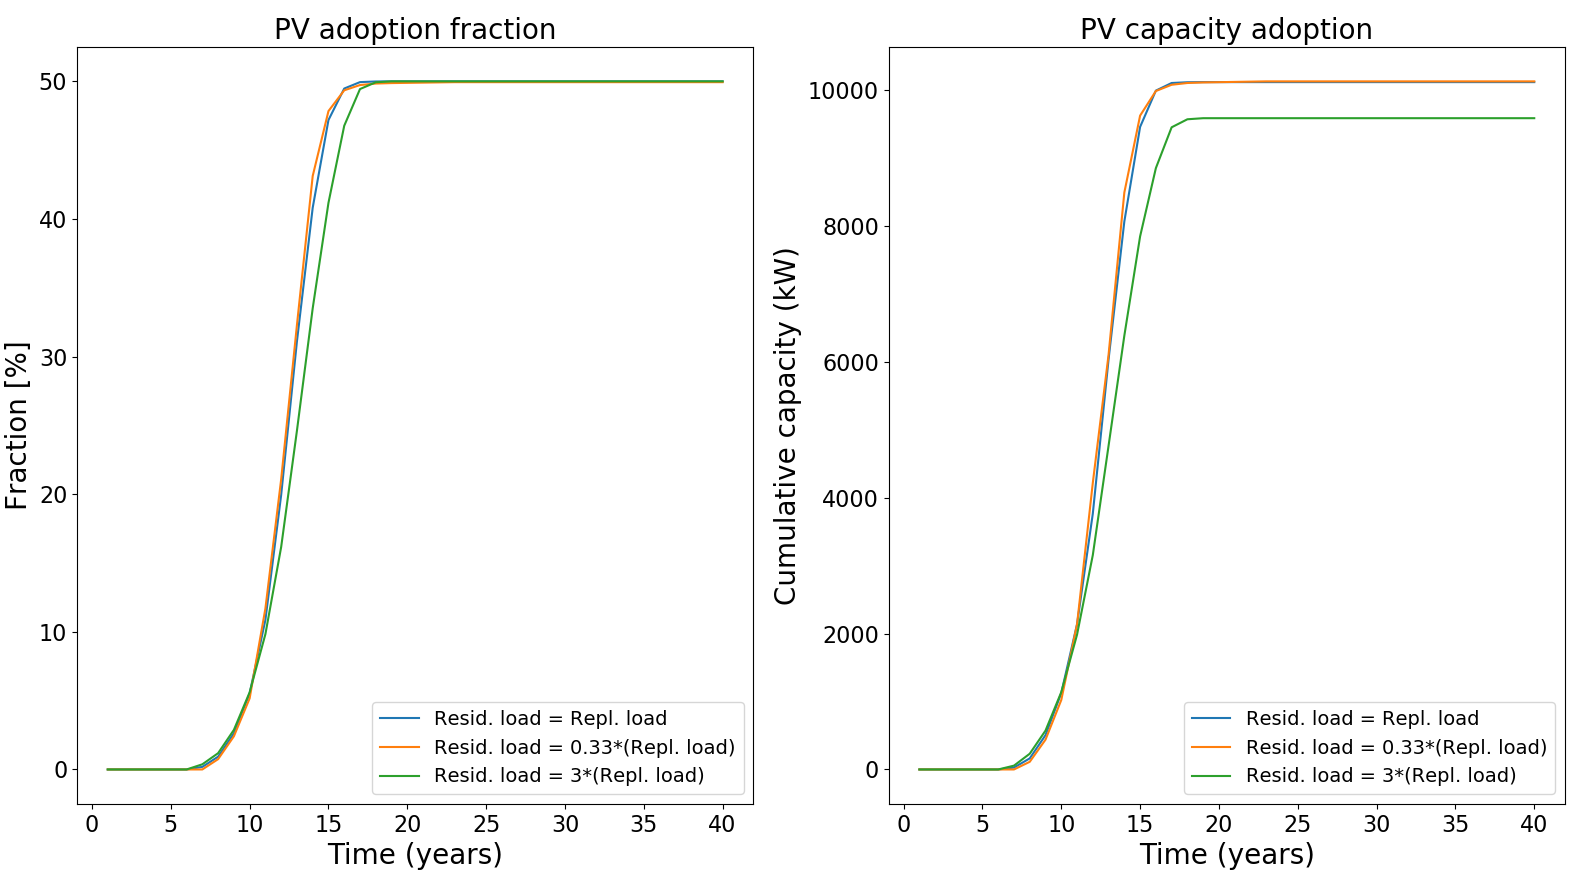
\includegraphics[width=12cm]{ModelAnalysis/PVresid.png}
\caption{PV adoption for different residual loads}
\label{Figure:pvresid}
\end{figure}
 \noindent
Here, the effect of different residual loads is quite subtle. The results for the three residual loads are quite similar, both in adoption fraction and in cumulative PV capacity adopted. The only exception is the cumulative PV capacity for the higher residual load, which will be slightly lower due to the lower savings. This also applies to the battery technology, although the cumulative capacity does show some more variation, as can be seen in Figure \ref{Figure:batresid}. For both technologies, the cumulative adopted capacity for the higher residual load will be lower since the savings will be lower. These savings will be lower because the DSO will have less recurring revenue to rely on, which will force him to adapt his tariffs more rapidly. For the higher residual load, the opposite effects will play. 
\begin{figure}[h!]
\centering
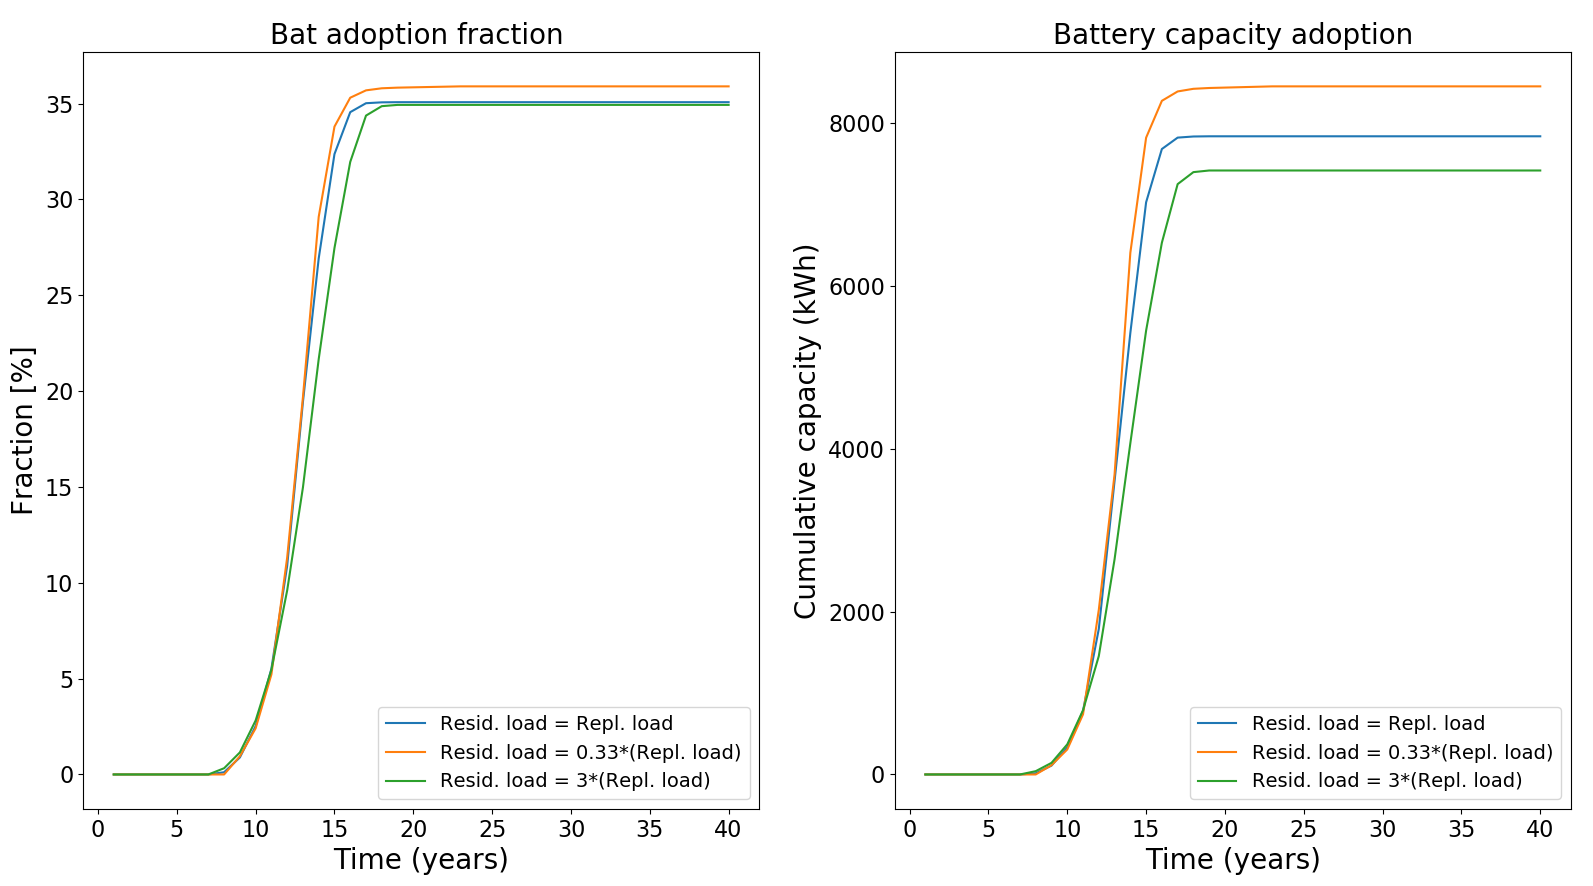
\includegraphics[width=12cm]{ModelAnalysis/BatResid.png}
\caption{Battery adoption for different residual loads}
\label{Figure:batresid}
\end{figure}
\noindent
The resulting configuration distribution can be seen in Figure \ref{Figure:configresid}. Here, the effect of different residual loads becomes more visible. For the lower residual loads, which translates into higher tariffs and savings, the largest configuration (4\textit{kW}/5\textit{kWh}) will become more popular. For the higher residual load, the tariffs and savings will be lower, making this configuration less popular. In fact, the change in battery adoption that can be seen in Figure \ref{Figure:batresid} is mainly due to the variation of this 5\textit{kWh} configuration.
In addition to the largest configuration, the variation of the residual load will also have an effect on smaller configurations, most notably the 1.5\textit{kW}/2\textit{kWh} installation. Contrary to the larger configurations, this one will become more popular in the high residual load case, when savings are lower, while being less popular in the low residual load case, when savings are higher. The resulting distribution tariff can be found in Figure \ref{Figure:distresid}. In parallel with the adoption levels, the distribution tariff will increase by more than 300\% in the low residual load case, while this increase will only be 33.1\% in the case of a higher residual load. 
\begin{figure}[h!]
\centering
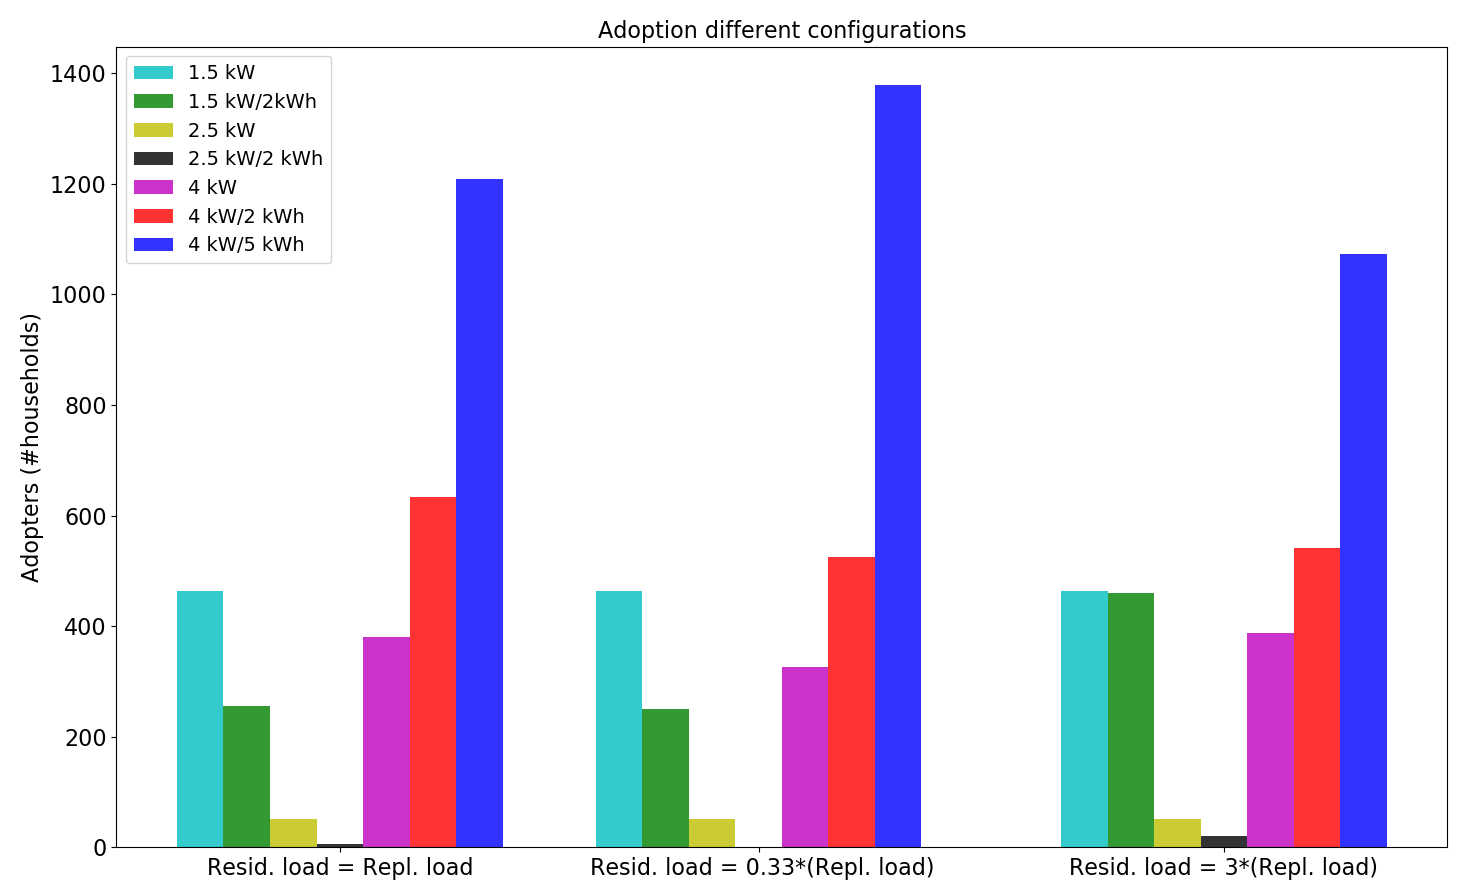
\includegraphics[width=12cm]{ModelAnalysis/ConfigResid.png}
\caption{Configurations for different residual loads}
\label{Figure:configresid}
\end{figure}
 \noindent
The resulting configuration distribution can be seen in Figure \ref{Figure:configresid}. Here, the effect of different residual loads becomes more visible. For the lower residual loads, which translates into higher tariffs and savings, the largest configuration (4\textit{kW}/5\textit{kWh}) will become more popular. For the higher residual load, the tariffs and savings will be lower, making this configuration less popular. In fact, the change in battery adoption that can be seen in Figure \ref{Figure:batresid} is mainly due to the variation of this 5\textit{kWh} configuration.
In addition to the largest configuration, the variation of the residual load will also have an effect on smaller configurations, most notably the 1.5\textit{kW}/2\textit{kWh} installation. Contrary to the larger configurations, this one will become more popular in the high residual load case, when savings are lower, while being less popular in the low residual load case, when savings are higher. The resulting distribution tariff can be found in Figure \ref{Figure:distresid}. In parallel with the adoption levels, the distribution tariff will increase by more than 300\% in the low residual load case, while this increase will only be 33.1\% in the case of a higher residual load. 
\newline \newline \noindent
The resulting distribution tariff can be found in Figure \ref{Figure:distresid}. In parallel with the adoption levels, the distribution tariff will increase by more than 300\% in the low residual load case, while this increase will only be 33.1\% in the case of a higher residual load.  
\begin{figure}[h!]
\centering
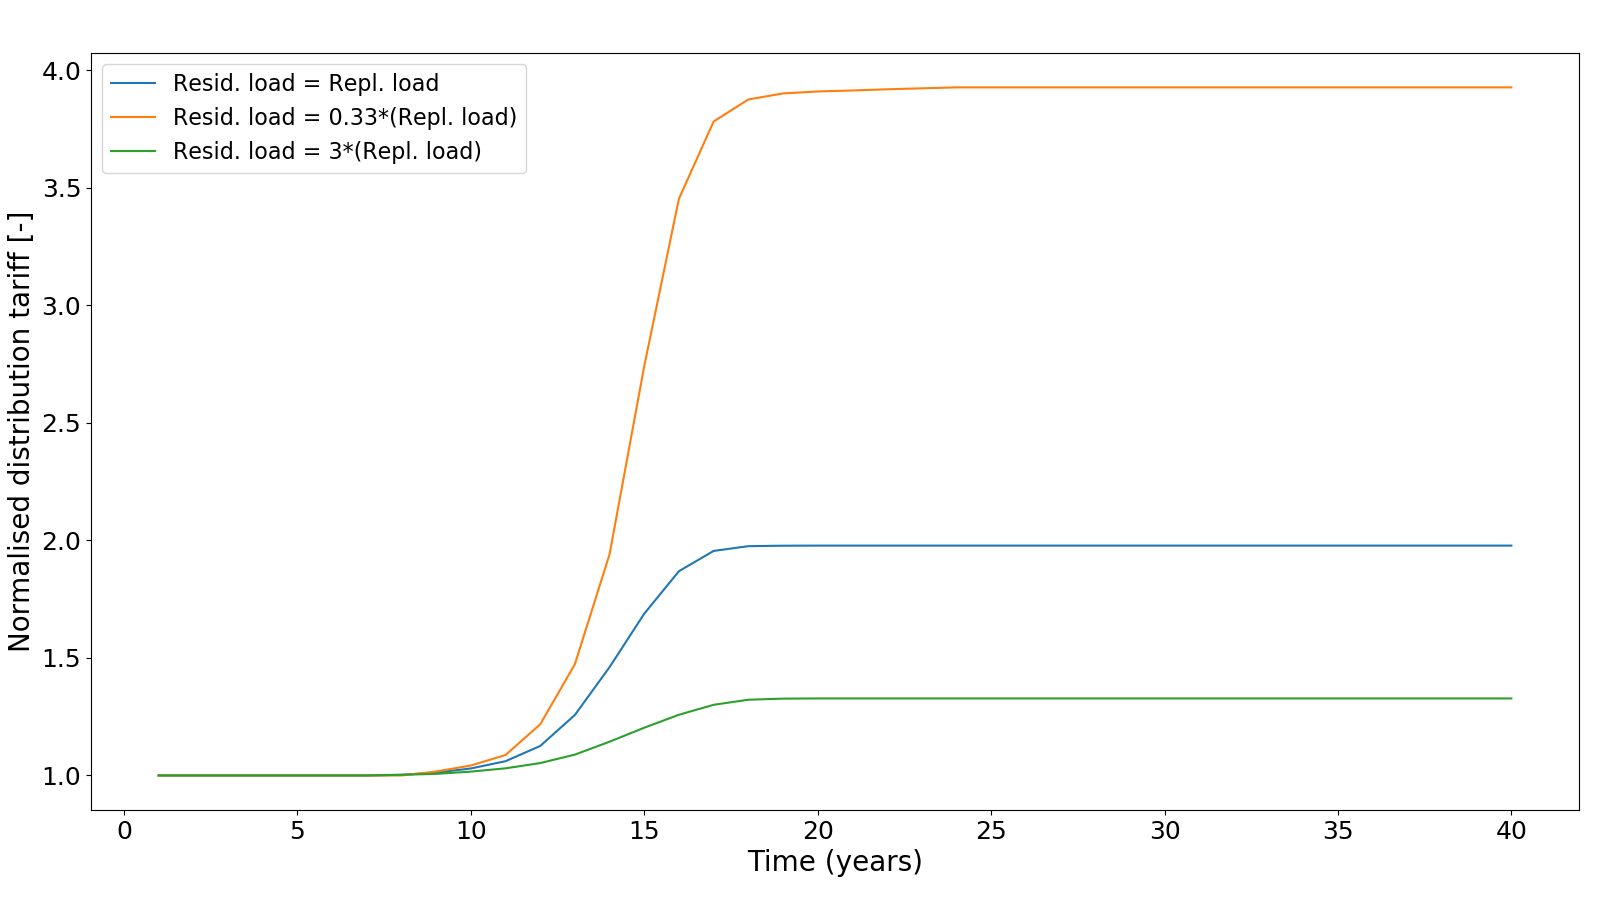
\includegraphics[width=10cm]{ModelAnalysis/distresid.png}
\caption{Distribution tariff for different residual loads}
\label{Figure:distresid}
\end{figure}
\noindent
Judging by the data presented in this section, the residual load has an effect on the adoption of certain configurations. Most notably, the adoption of the 1.5\textit{kW}/2\textit{kWh} and 4\textit{kW}/5\textit{kWh} configurations will change as a function of the residual load. This is mainly due to the effect of a change in the network charge on the savings. The lower the residual load, the more popular the large configurations and the less popular the small configurations will be. The higher the residual load, the more popular the smaller configurations are and the less popular the larger configurations. This adoption shift between different configurations will cause the effect on the aggregate adoption fraction and capacity adopted to be rather limited, with the exception of the battery capacity adopted. In parallel with the DER evolution, the network charges will increase in the utility death spiral process. 

\subsection{Network charge}
\label{distanal} As was already discussed in Section \ref{compar}, the different network charges have a different effect on the savings and, therefore, the overall adoption and subsequent utility death spiral. The main driver for this difference in adoption between the net volumetric tariff and annual capacity offtake tariff is the difference in savings between the two tariffs. Both the way in which savings are created as well as the effect of this change in savings on the adoption of DER will be discussed in the next few paragraphs.
\newline \newline \noindent
Since the savings for a household due to the adoption of DER consist of both energy costs and (some) distribution costs, the overall savings will evolve with these components. In the case of the net volumetric distribution tariff, the distribution component can be calculated using Equation \ref{distnet}. This cost formula suggest that the savings of the household can increase substantially in case $q_{net}$ reaches a value close to zero. As can be seen in Figure \ref{Figure:netdem}, $q_{net}$  of all but two configurations is equal to zero, meaning that all distribution charges are avoided. Compared to $q_{net}$ for no DER adoption, the savings of the distribution component and by extension the electricity cost are significant. 
\begin{figure}[h!]
\centering
\includegraphics[width=12cm]{ModelAnalysis/Netdemand.png}
\caption{Net volumetric demand for different DERs configurations}
\label{Figure:netdem}
\end{figure}
\noindent
For the annual capacity offtake tariff, the distribution cost can computed using Equation \ref{qcap}. This network charge formulation suggests that, like in the volumetric case, the distribution cost could decrease to zero. When looking at Figure \ref{Figure:peakdem}, however, it becomes clear that $q_{cap}$ and the distribution cost component will remain strictly positive for all configurations.  
\begin{figure}[h!]
\centering
\includegraphics[width=12cm]{ModelAnalysis/PeakDemand.png}
\caption{Different peak demands}
\label{Figure:peakdem}
\end{figure}
\noindent
Due to the previously discussed difference in distribution cost for the two different network charges, the savings will de different, as can be seen in Figure \ref{Figure:Savings} \footnote{The represented data is the average of the savings for all configurations}. Here, it can be seen how the savings realised in the case of the net volumetric distribution tariff are much higher than for the annual capacity offtake tariff. Besides having a larger initial value, the savings for the volumetric network charge also increase more streadily than those in the capacity tariff case: the volumetric savings increase by 39.6\% throughout 40 year simulation, whereas they only increase by 6.8\% in the capacity case pver the same period. This is a direct result of the higher initial value in the volumetric distribution tariff case: the higher savings cause a higher adoption incentive, causing the utility death spiral to manifest itself more clearly, which will cause the distribution tariff to increase further. The results discussed in Section \ref{compar} showed the extent of this utility death spiral for the different policies. 
\begin{figure}[h!]
\centering
\includegraphics[width=12cm]{ModelAnalysis/Savings.png}
\caption{Savings for the volumetric and capacity tariff}
\label{Figure:Savings}
\end{figure}
\subsection{Preliminary analysis \& Conclusion}
What also became clear from this analysis, is the role of the residual load in the DER adoption process. Since a lower residual load causes the network charges and savings to be higher, the incentive to adopt DER becomes higher, thereby reinforcing the network charge increase once again, creating a vicious circle. Currently, the fraction of DER in the overall electricity landscape still is limited, but rising quickly. Over the next few decades, as policy makers intend to make a large portion of the households adopt DER to reduce emissions, the residual load will become a smaller portion of the overall load, which would cause the utility death spiral effects to be amplified. The distribution cost evolution for low residual loads that was presented in Figure \ref{Figure:distresid} could, therefore, materialize over the next few decades if appropriate action is not taken. As was discussed in Section \ref{compar}, the capacity-based network charge can mitigate these effects. The main reason for this, as was discussed in Section \ref{distanal}, is the change in the distribution cost component and its effects on the savings and adoption incentive. For the net volumetric distribution tariff, this cost component decreases to zero for most configurations, generating more savings to the households and encouraging DER adoption. The design of the capacity offtake tariff, however, will cause the distribution component to decrease by a smaller amount for most configurations, generating less savings to the households, thereby encouraging DER adoption to a lesser extent. 
\newline \newline \noindent
\section{Discussion \& Future work} \label{future}
In previous sections, the results of the model were discussed in order to address the main research question and the complementary sub-questions of this Thesis. The discussion was separated according to these research questions. The first research question related to the evaluation of different policies with regards to the DER adoption and utility death spiral. The main takeaways here are:
\begin{itemize}
\item The net billing policy can serve as an efficient way to encourage rapid adoption of small DER configurations. These installations will predominantly serve the inflexible demand of the households and inject a limited amount of electricity into the grid. This will cause less grid stability issues, but due to the lower aggregate renewable energy produced, there will be less grid decarbonisation. 
\item The net metering policy and additional battery subsidies can serve as a way to encourage a large cumulative adoption capacity of DER installations. These policies will, however, cause larger amounts of grid injection. Their efficiency is, therefore, questionable if the intention of the policy makers is to encourage self-consuming households. If policy makers intend to maximize the energy production of the installed DER for operation or decarbonization purposes, the net metering and battery subsidy policy are suitable incentive programs.
\item The net volumetric distribution tariff will encourage larger and quicker adoption of PV and batteries due to larger savings. In parallel, the utility death spiral (i.e. tariff modification by the DSO) will manifest itself more clearly. The capacity offtake tariff, on the other hand, can partially mitigate the effects on this utility death spiral while still ensuring widespread PV and limited battery adoption, be that over a longer period of time. In the future grid, where widespread DER adoption and the subsequent utility death spiral are extremely likely prospects, this network charge is the clear favorite. 
\end{itemize}
Given this difference between the policies, governments and policy makers must clearly identify their objectives (DER adoption, utility death spiral mitigation, etc.) before choosing what incentive program to put into action. The first research sub-question relates to the sensitivity of certain parameters embedded in the model. 
\begin{itemize}
\item The selected value for the loss aversion coefficient ($\lambda = 1.5$) and risk aversion ($\alpha = \beta = 0.6$) can provide a consistent set of results and suggests that future research into adequate values of this parameter can add valuable insights. 
%\item The lower the residual load the DSO can rely on, the more the utility death spiral will manifest itself. In the future grid, where DER adoption becomes more pervasive, this effect will become increasingly present and is a threat that must be anticipated. The capacity tariff is a means to mitigate this utility death spiral effect.
\item Battery subsidies can help encourage the adoption of residential batteries, but the main effect of these subsidies is the increased adoption of the largest configurations available, causing large-scale grid injection. Given the amount of government resources these subsidy programs require, this subsidy may not be necessary if the battery technology sufficiently expands and scales in cost in the near future, since the battery cost reduction also is an important driver in the battery adoption process. 
\end{itemize}
The second research sub-question relates to the comparison of the model results with the EUT.
\begin{itemize}
\item  CPT as a decision-making theory to simulate the adoption of DER in consumer-centric energy systems can complement the results provided by the EUT.
\item The results of EUT compared to the CPT are cruder and less refined, since the adoption does not follow the same adoption trend and tends to focus the adoption or one of two configurations. For the annual net metering case, the adoption focuses on the smallest configurations, without any batteries, whereas this focus completely shifts to two medium-to-large PV-battery configurations for the annual capacity offtake case. 
\item Despite the uncertainty concerning some of the parameters in CPT, like the loss aversion, risk aversion and reference levels, this theory can capture more complex behavior of a group of decision makers, like being able to describe a more diverse configuration adoption.
\end{itemize}
\newline \newline \noindent
Despite these valuable insights, further work still needs to be done in this field. First and foremost, since this Thesis attempted to provide qualitative insights into this novel approach to the simulation of DER adoption by using CPT, a test case must be performed to relate these insights to real-world results. This must be complemented by field experiments where energy prosumers are the target, in order to measure an accurate value of the loss aversion, risk aversion and reference levels. In addition, a number of additional items need further elaboration:
\begin{itemize}
\item Since the utility calculation only considers economic welfare and the peer effect, additional factors like advertisements, household profiles etc. must be considered in the utility calculation.
\item Some implicit assumptions made concerning the behavior of the households, like the absence of the rebound effect and the indifference of the residual households towards the increase in distribution tariffs, must be elaborated upon.
\item Since the diversification of the household was limited to the financial wealth of the household, this diversification must be elaborated to social, geographical and cultural factors influencing the nature of the households and his position towards DER adoption under uncertainty.
\item The assumption of constant weighting coefficients and the constant adoption nature of the different households must be elaborated to a situation where these parameters also become endogenous to the model and change over time: initially the economic weighting coefficient should be larger, but as the adoption proceeds over time, the peer effect weighting coefficient should be larger. In parallel, the number of innovators and laggards could also change as a function of time and the adoption rates.
\item Whereas this Thesis considers the different policies separately, various combinations of the presented policies should be examined to find an optimal structure that can combine the positive effects of the respective policies while minimizing the negative effects of these programs. An example could be a policy that combines the quick adoption rates of the net billing policy with the limited utility death spiral effects of the annual capacity offtake policy. 
\item In addition to the parameters tested in the model, the time preference behavior of the households, which is captured through the discount factor, must be included in the model analysis. In doing so, this must be related to the loss aversion of the households to test different configurations of this behavior. 
\end{itemize}
Despite these items that need further work in this field, the results in this chapter have made a strong case for further research into CPT in an ABM framework for the simulation of DER adoption in a consumer-centric energy system, which was assumed to be a CAS. 
    
\chapter{Conclusion}
    

% Indien er bijlagen zijn:
\appendixpage*          % indien gewenst
\appendix
\chapter{Sensitivity analysis other policies}
\label{app:2}
In this Appendix, the sensitivity analysis of the parameters discussed in Section \ref{analysis} will be presented for the remaining policies: battery subsidies, net billing and the annual offtake capacity tariff. 
\section{Residual load}
\subsection{Battery subsidies}
The data for the residual load sensitivity analysis of the battery subsidy policy (combined with the net metering policy) can be found in Figures \ref{fig:M}, \ref{fig:N}, \ref{fig:O} and \ref{fig:P}. 
\newline 
\begin{figure}[h!]
    \centering
    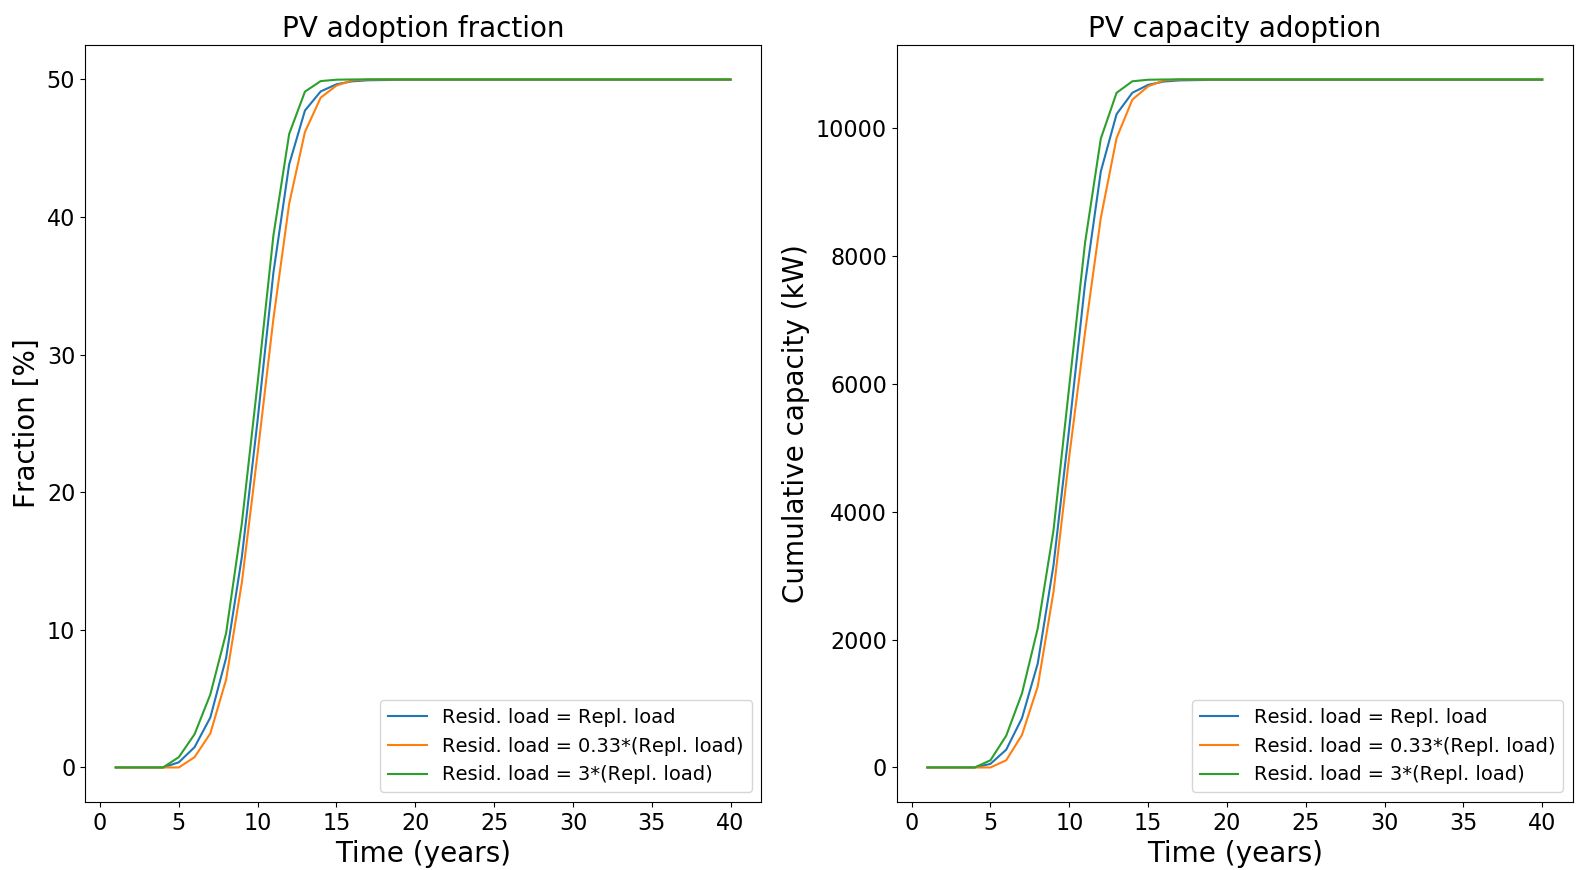
\includegraphics[width=10cm]{AppendixA/PVSubsresid.PNG}
    \caption{PV adoption for different residual loads}
    \label{fig:M}
\end{figure}
\noindent
\newline 
\begin{figure}[h!]
    \centering
    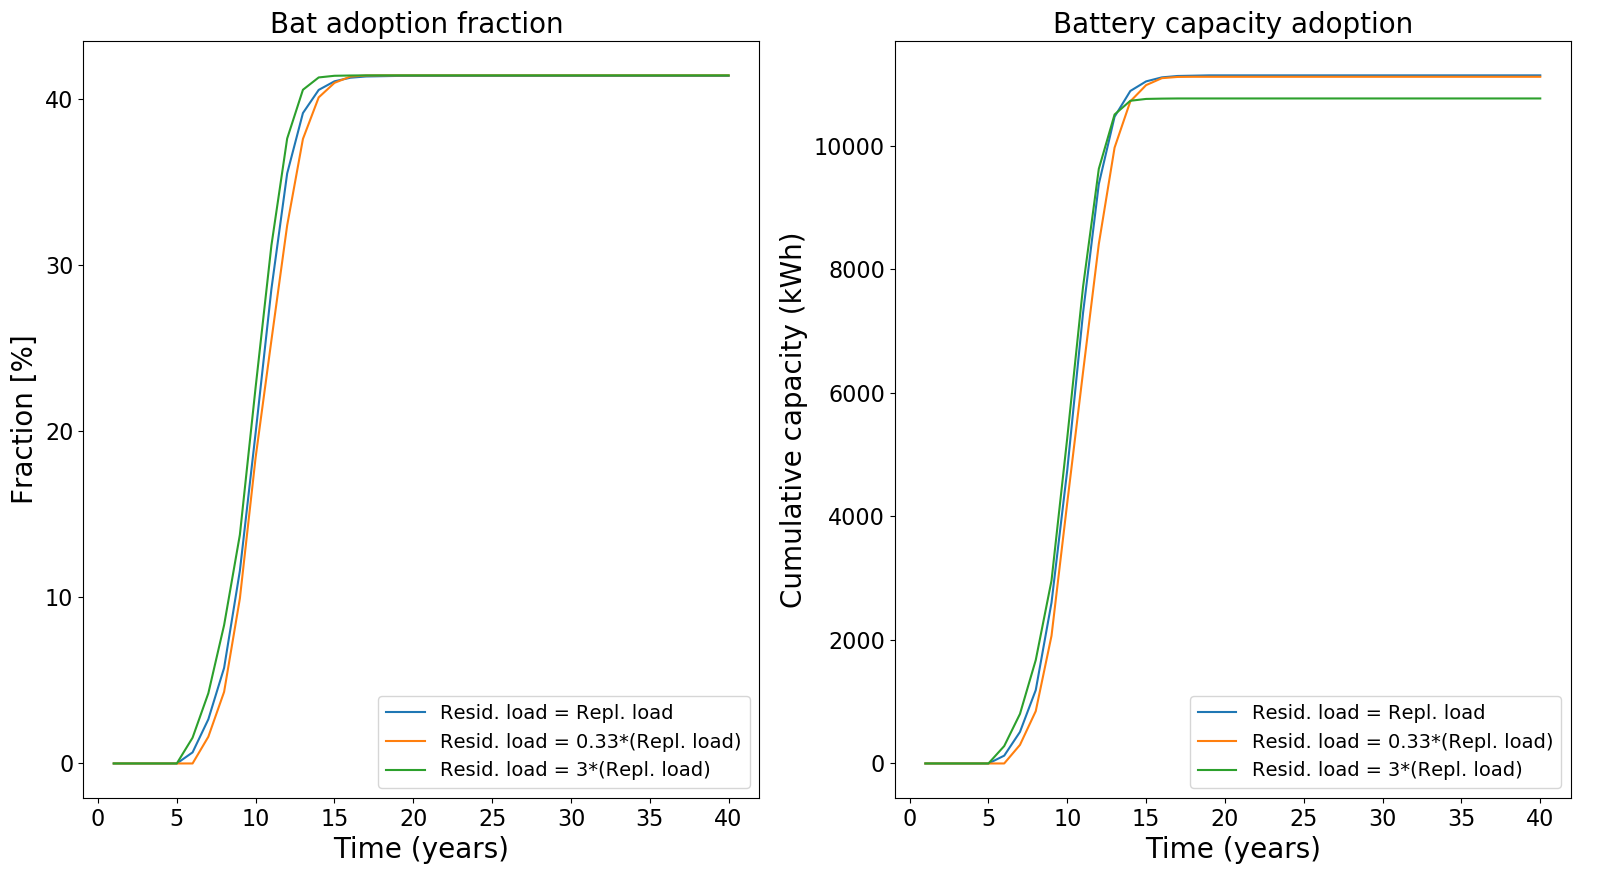
\includegraphics[width=10cm]{AppendixA/BatSubsresid.PNG}
    \caption{Battery adoption for different residual loads}
    \label{fig:N}
\end{figure}
\noindent
\newline 
\begin{figure}[h!]
    \centering
    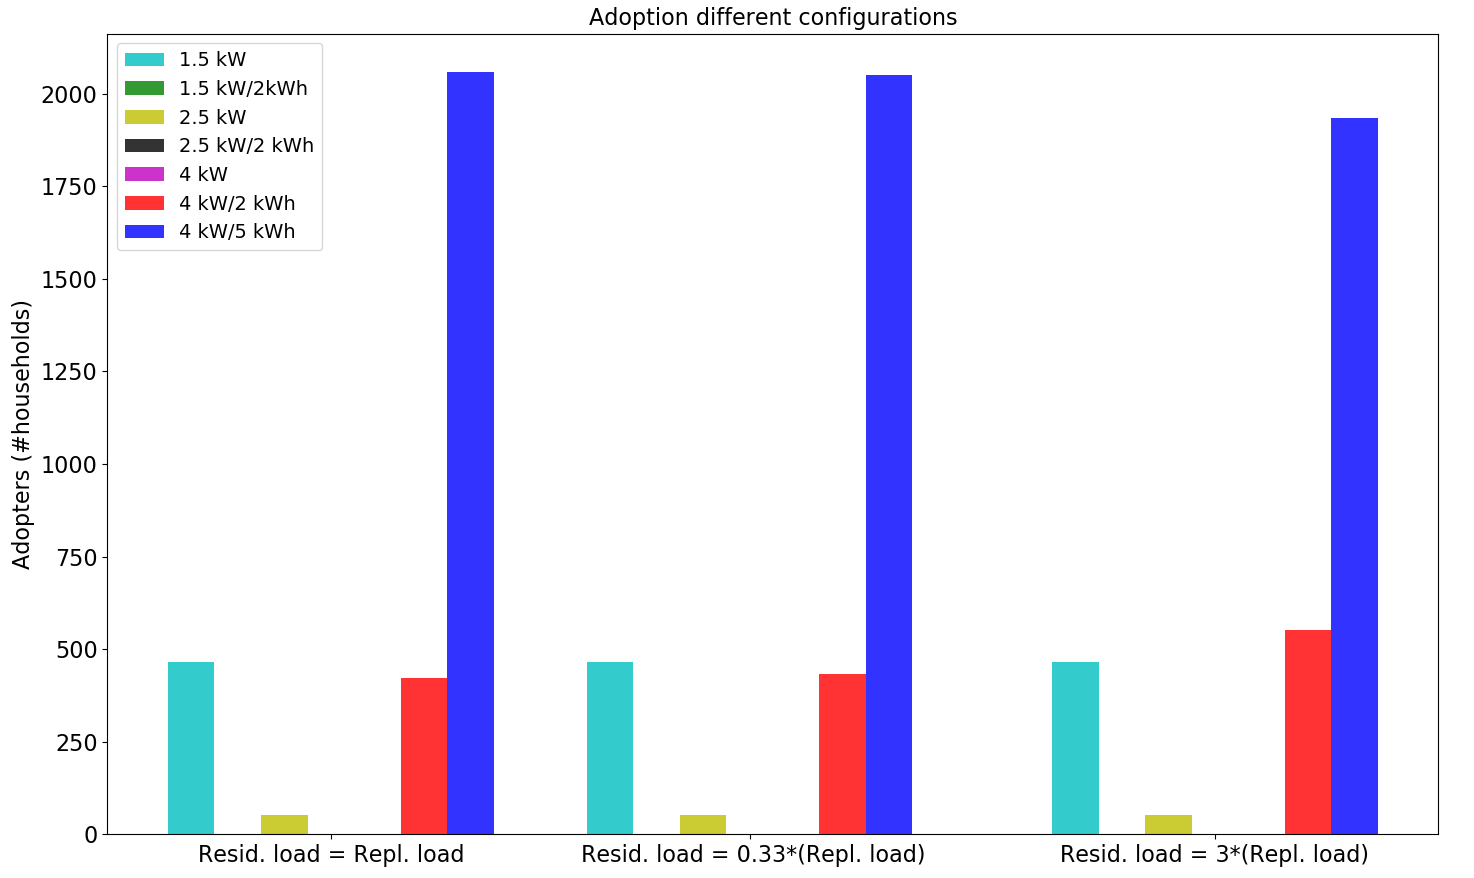
\includegraphics[width=10cm]{AppendixA/ConfigSubsresid.PNG}
    \caption{Configurations for different residual loads}
    \label{fig:O}
\end{figure}
\noindent
\newline
\begin{figure}[h!]
    \centering
    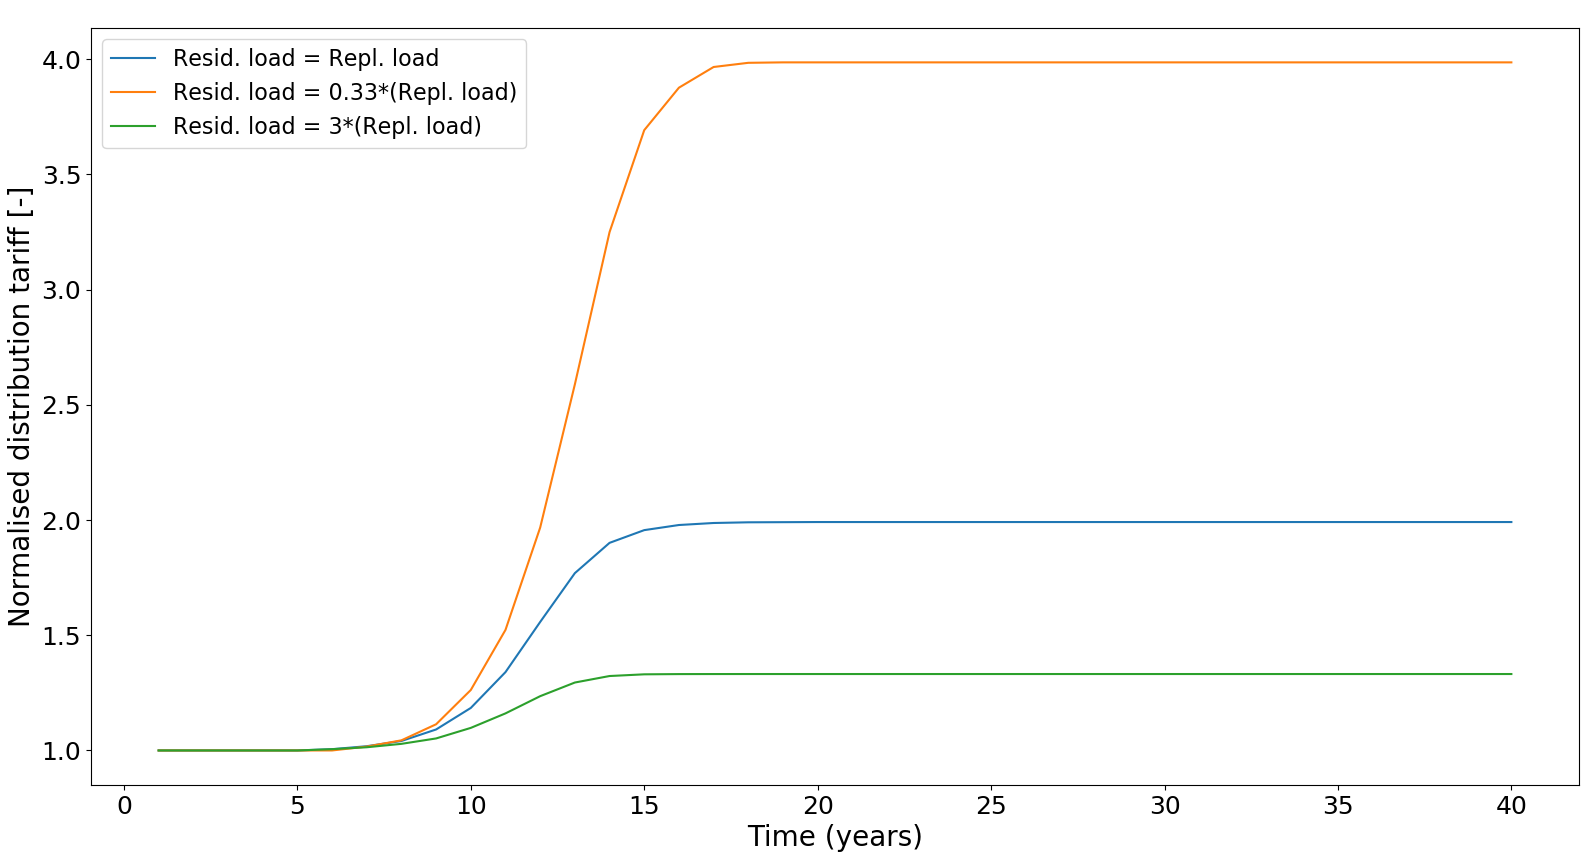
\includegraphics[width=10cm]{AppendixA/DistSubsresid.PNG}
    \caption{Normalised capacity tariff for different residual loads}
    \label{fig:P}
\end{figure}
\subsection{Net billing}
The data for the residual load sensitivity analysis of the net billing policy can be found in Figures ref{fig:R}, %\ref{fig:S}, \ref{fig:T} and \ref{fig:U}. 
\newline 
\begin{figure}[h!]
    \centering
    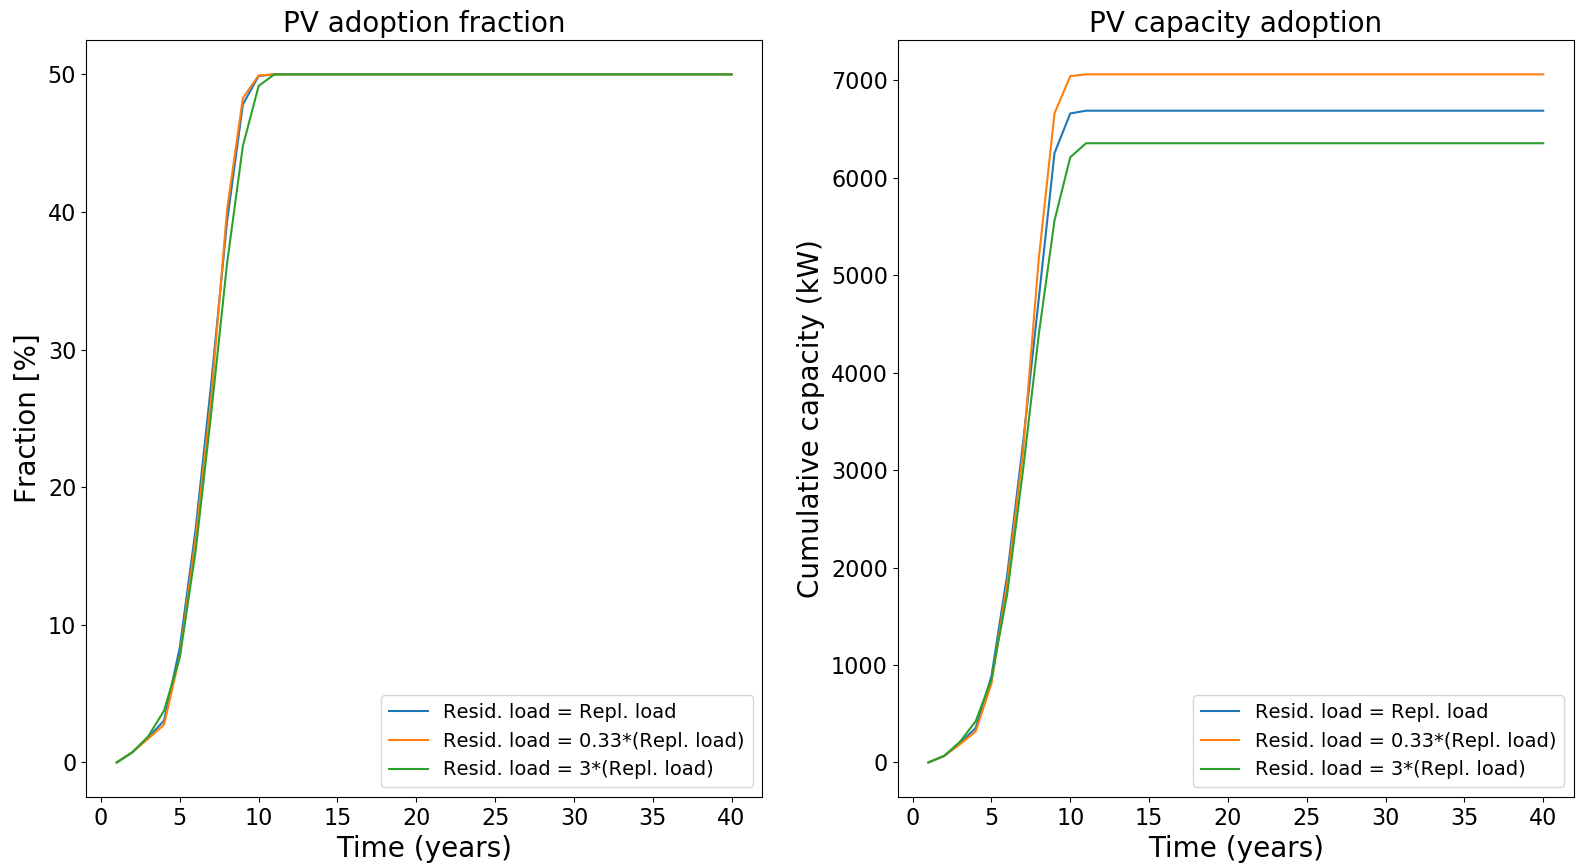
\includegraphics[width=10cm]{AppendixA/PVNBresid.PNG}
    \caption{PV adoption for different residual loads}
    \label{fig:Q}
\end{figure}
\noindent
\newline 
\begin{figure}[h!]
    \centering
    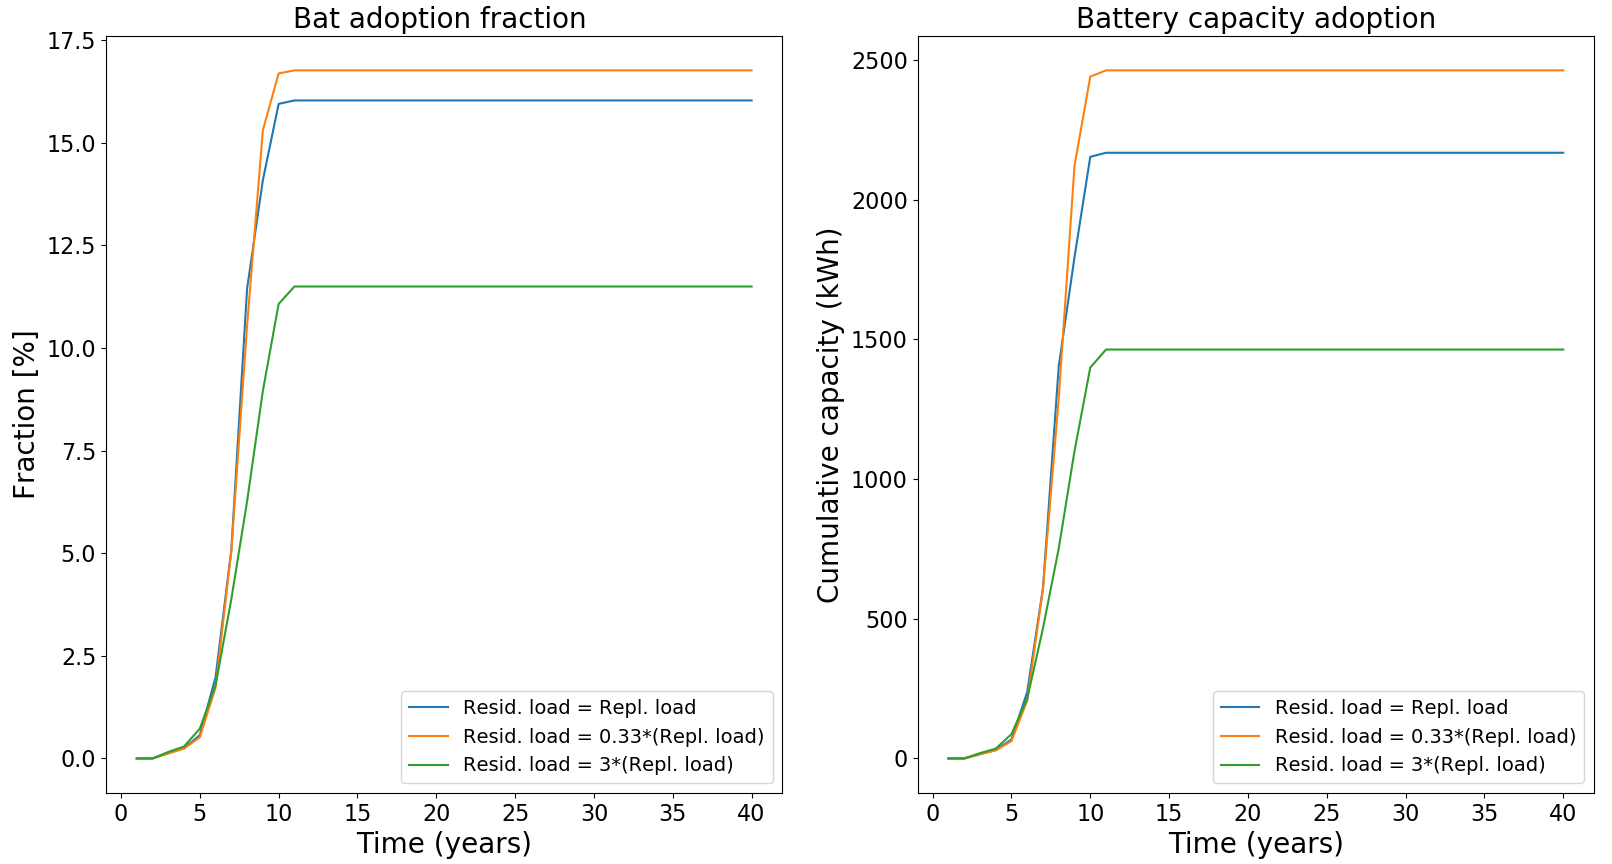
\includegraphics[width=10cm]{AppendixA/BatNBresid.PNG}
    \caption{Battery adoption for different residual loads}
    \label{fig:R}
\end{figure}
\noindent
\newline 
\begin{figure}[h!]
    \centering
    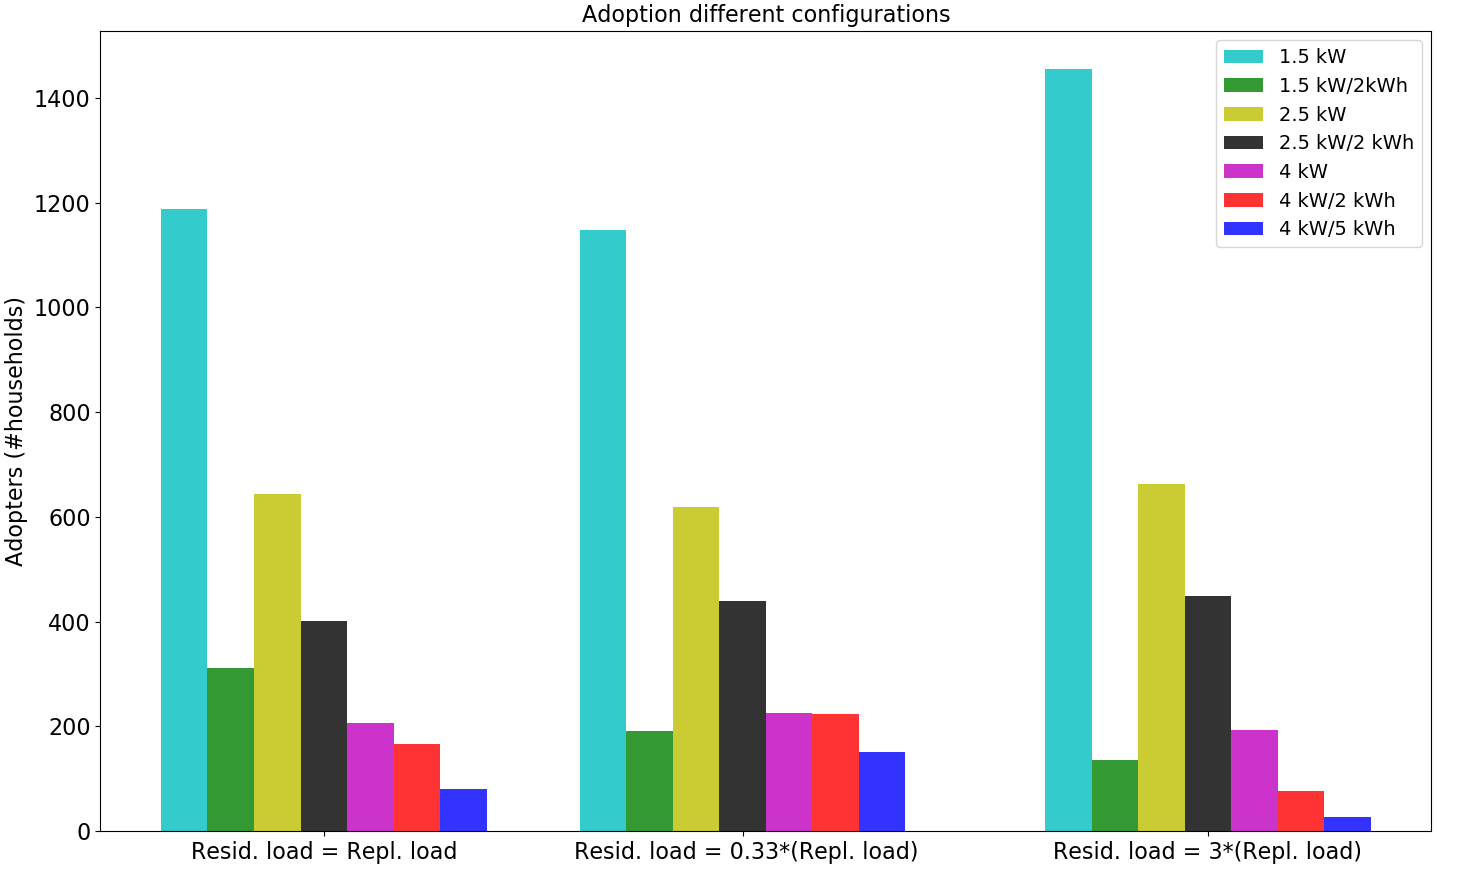
\includegraphics[width=10cm]{AppendixA/ConfigNBresid.PNG}
    \caption{Configurations for different residual loads}
    \label{fig:S}
\end{figure}
\noindent
\newline
\begin{figure}[h!]
    \centering
    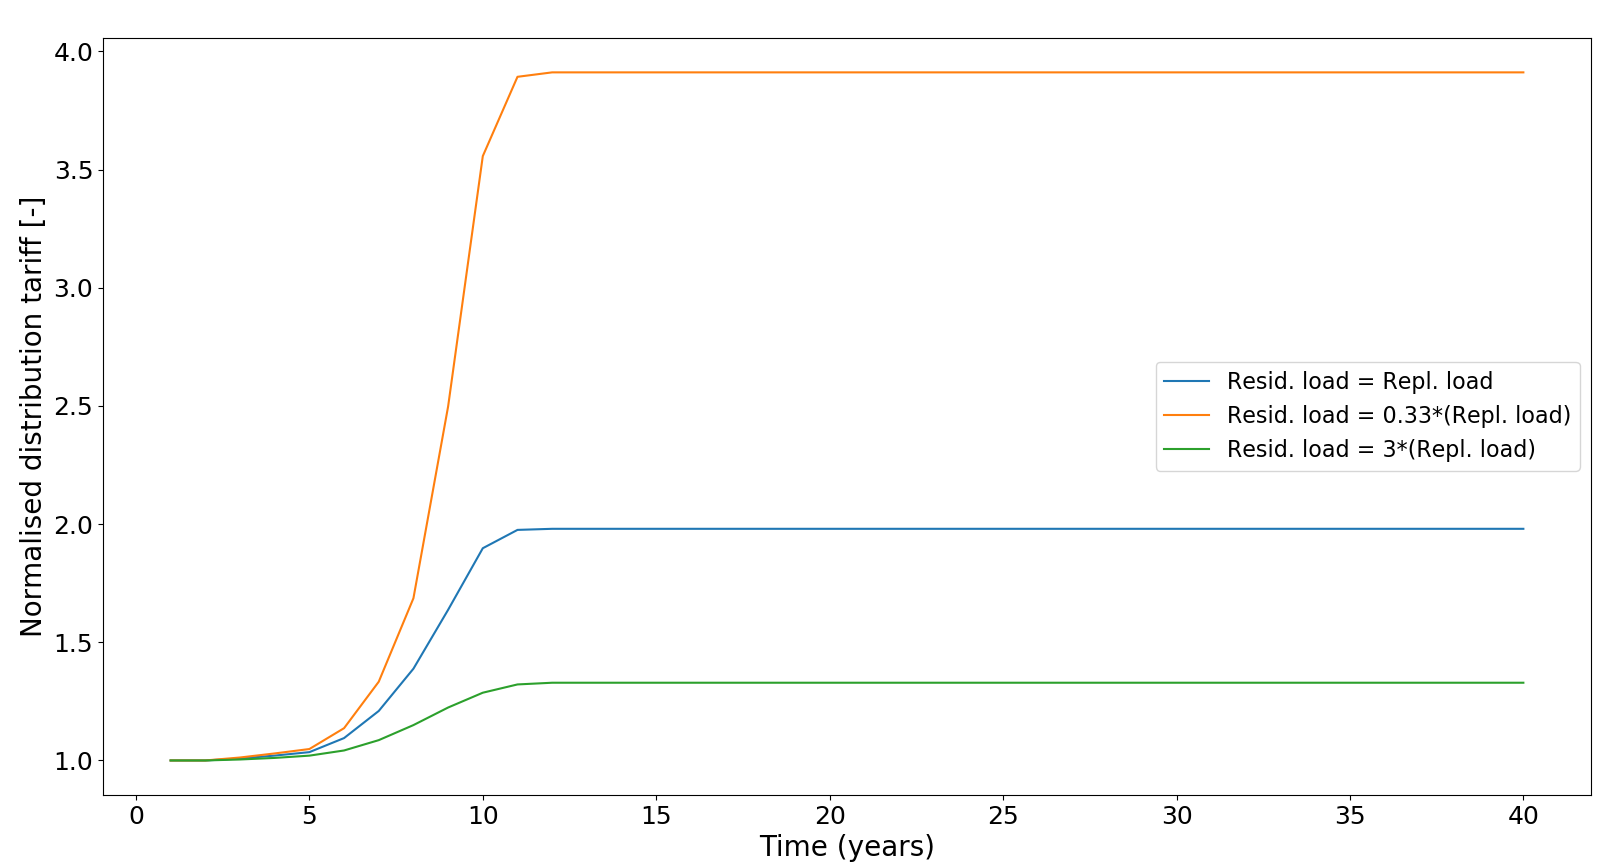
\includegraphics[width=10cm]{AppendixA/DistNBresid.PNG}
    \caption{Normalised capacity tariff for different residual loads}
    \label{fig:T}
\end{figure}
\subsection{Annual capacity offtake}
The data for the residual load sensitivity analysis of the annual capacity offtake 
\newline 
\begin{figure}[h!]
    \centering
    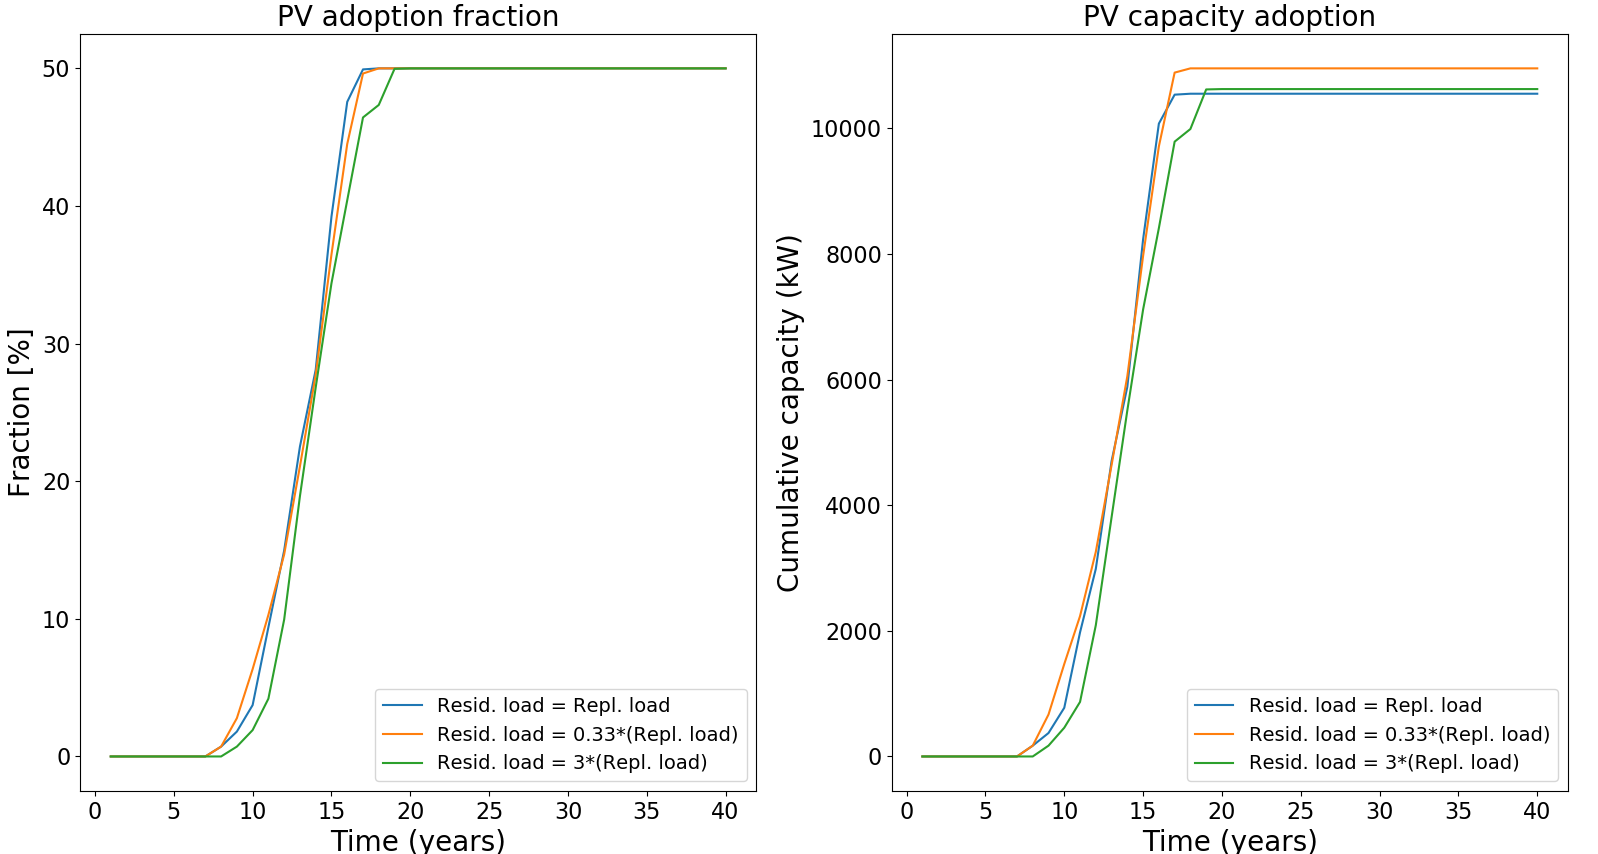
\includegraphics[width=10cm]{AppendixA/PVCapresid.PNG}
    \caption{PV adoption for different residual loads}
    \label{fig:U}
\end{figure}
\noindent
\newline 
\begin{figure}[h!]
    \centering
    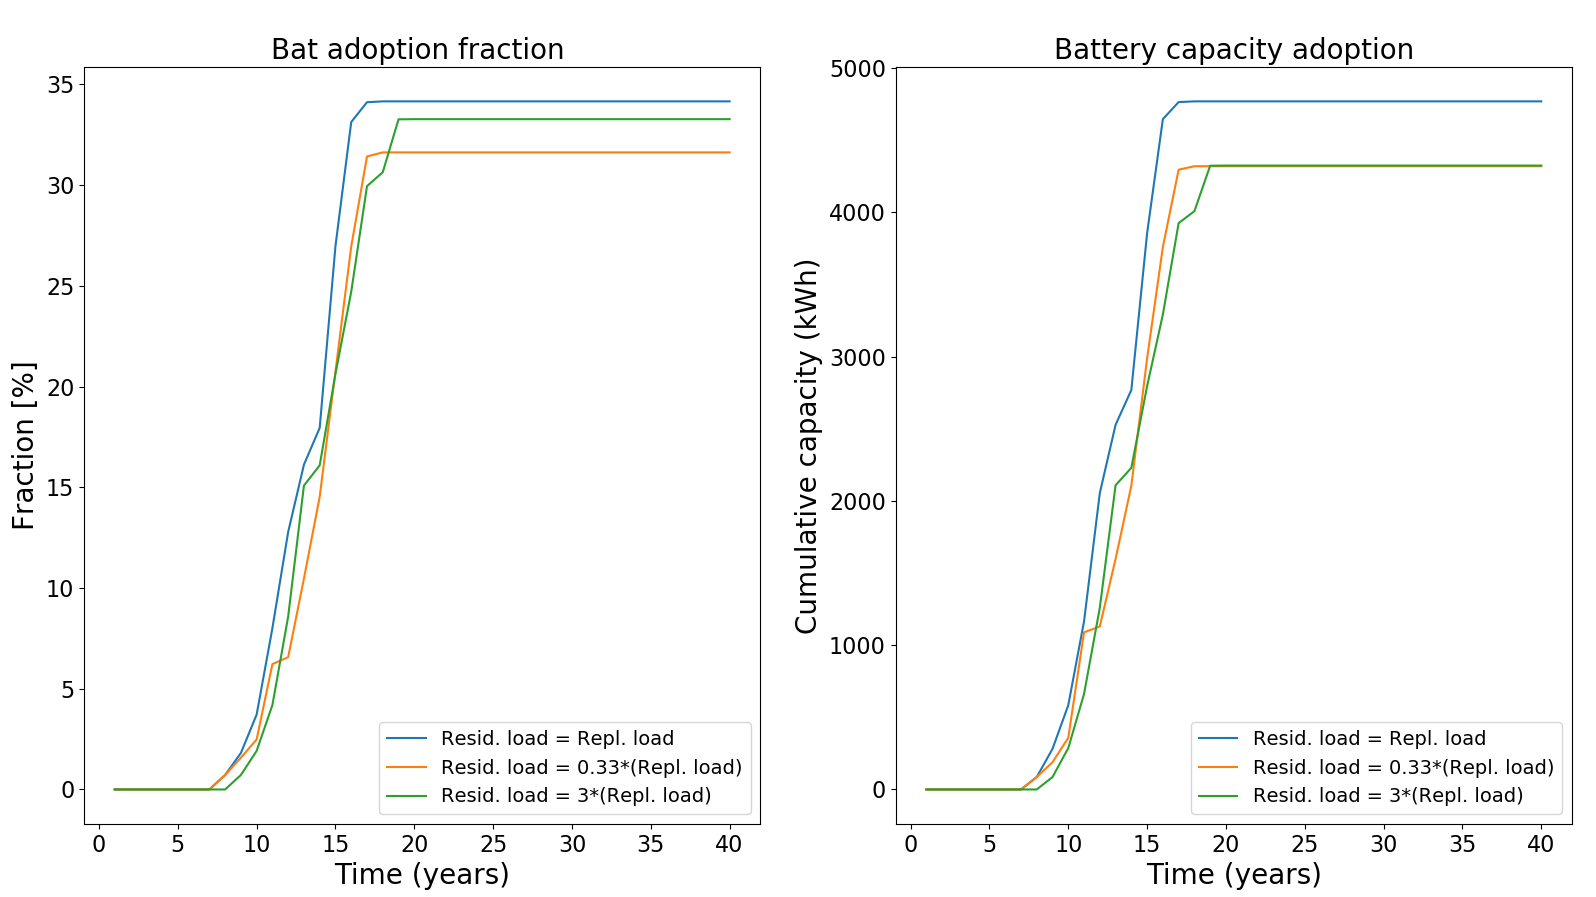
\includegraphics[width=10cm]{AppendixA/BatCapresid.PNG}
    \caption{Battery adoption for different residual load}
    \label{fig:V}
\end{figure}
\noindent
\newline 
\begin{figure}[h!]
    \centering
    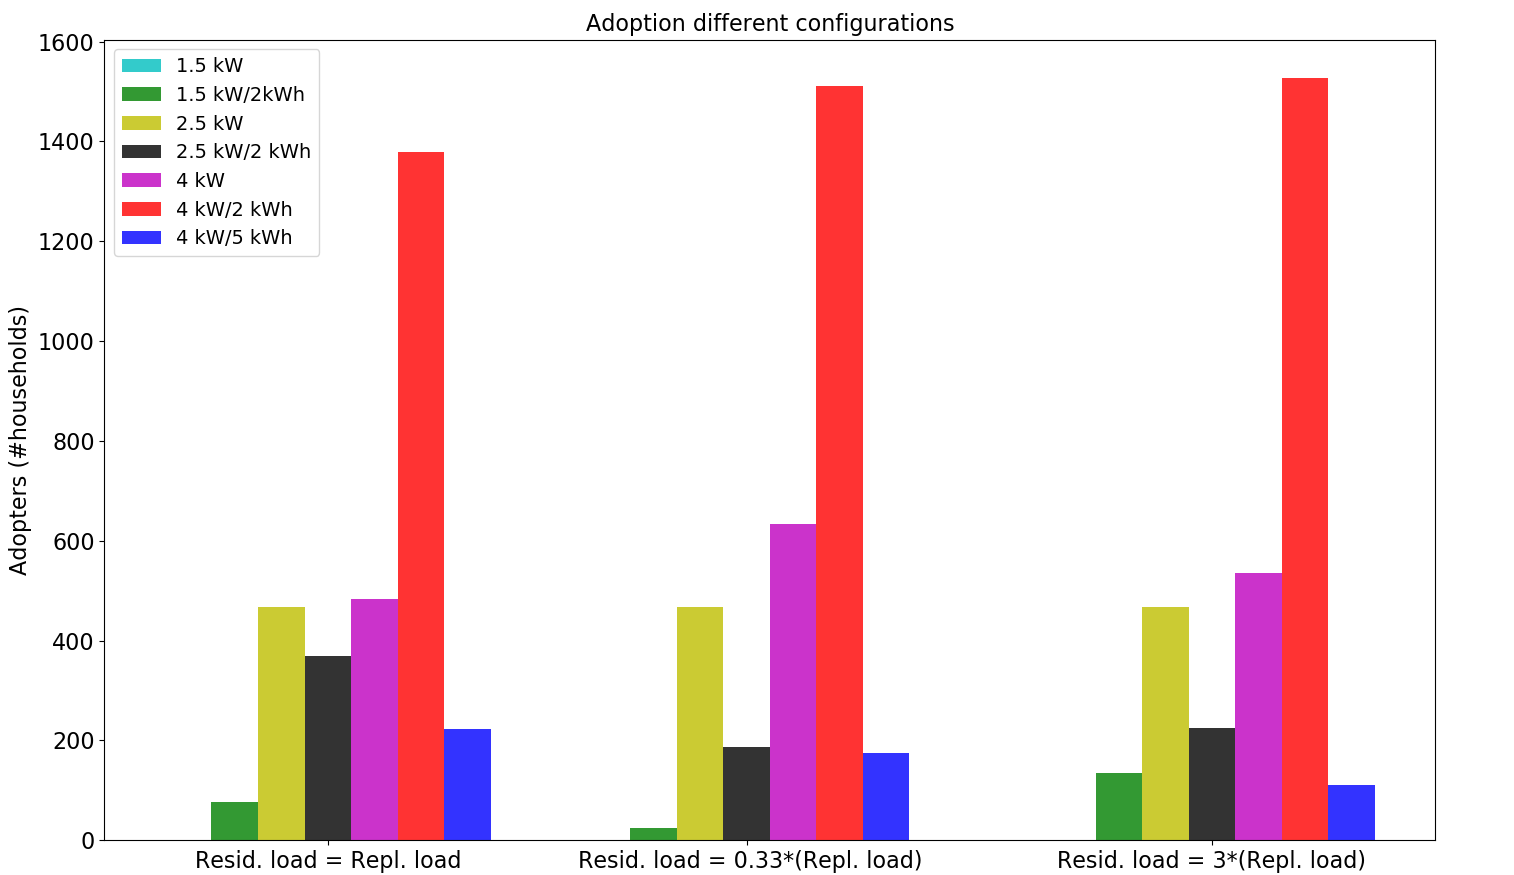
\includegraphics[width=10cm]{AppendixA/ConfigCapresid.PNG}
    \caption{Configurations for different residual loads}
    \label{fig:W}
\end{figure}
\noindent
\newline
\begin{figure}[h!]
    \centering
    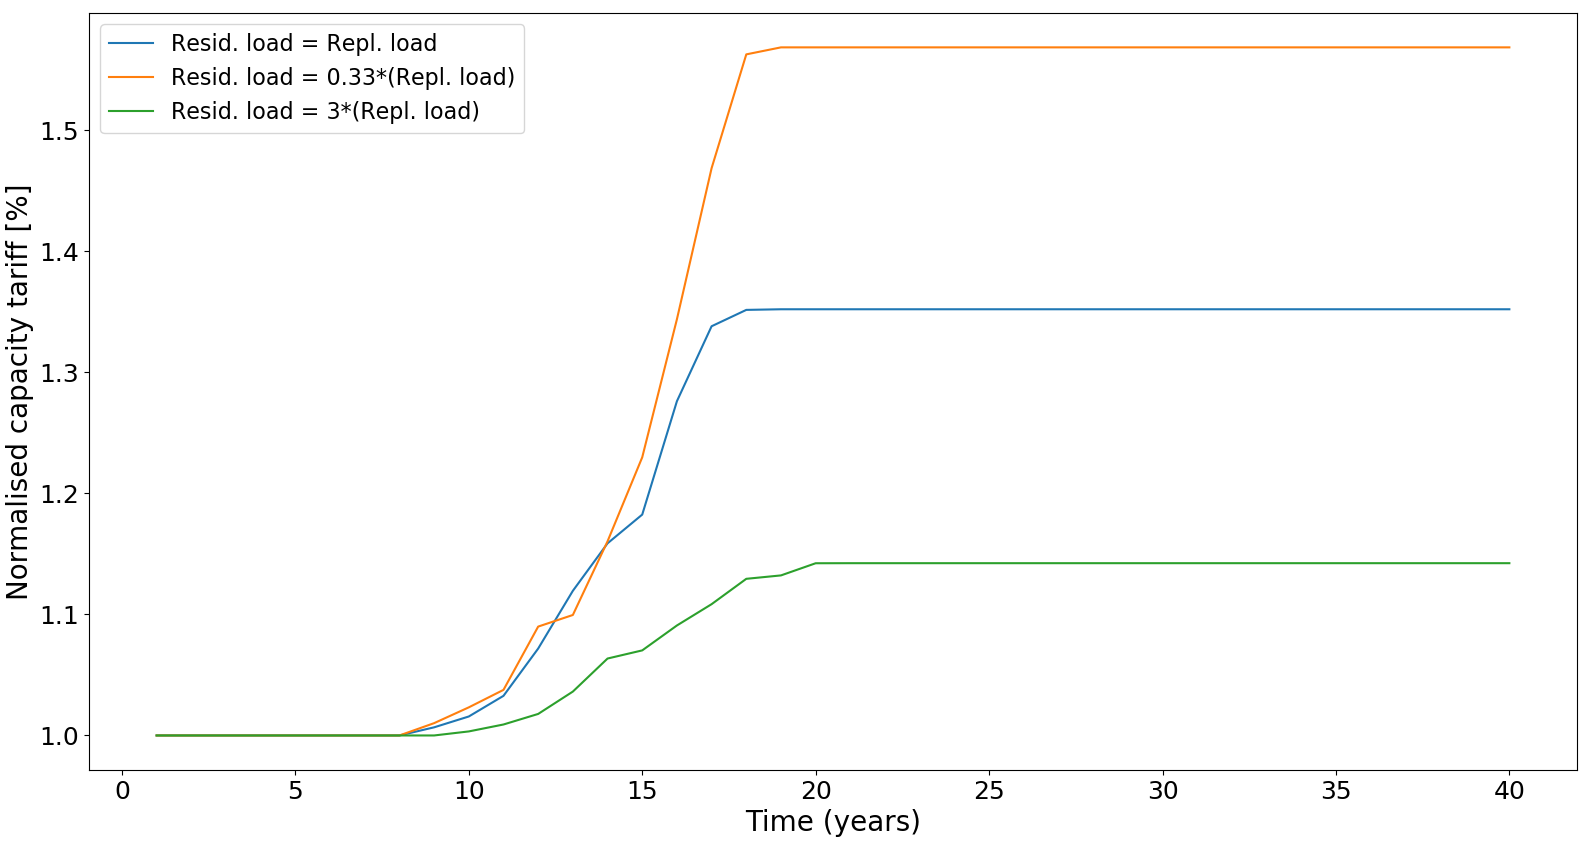
\includegraphics[width=10cm]{AppendixA/CapTarresid.PNG}
    \caption{Normalised distribution tariff for different residual loads}
    \label{fig:X}
\end{figure}
\section{Battery subsidies}
\subsection{Annual capacity offtake}
The data for the loss aversion sensitivity analysis of the battery subsidy policy (combined with the net metering policy). 
\newline 
\begin{figure}[h!]
    \centering
    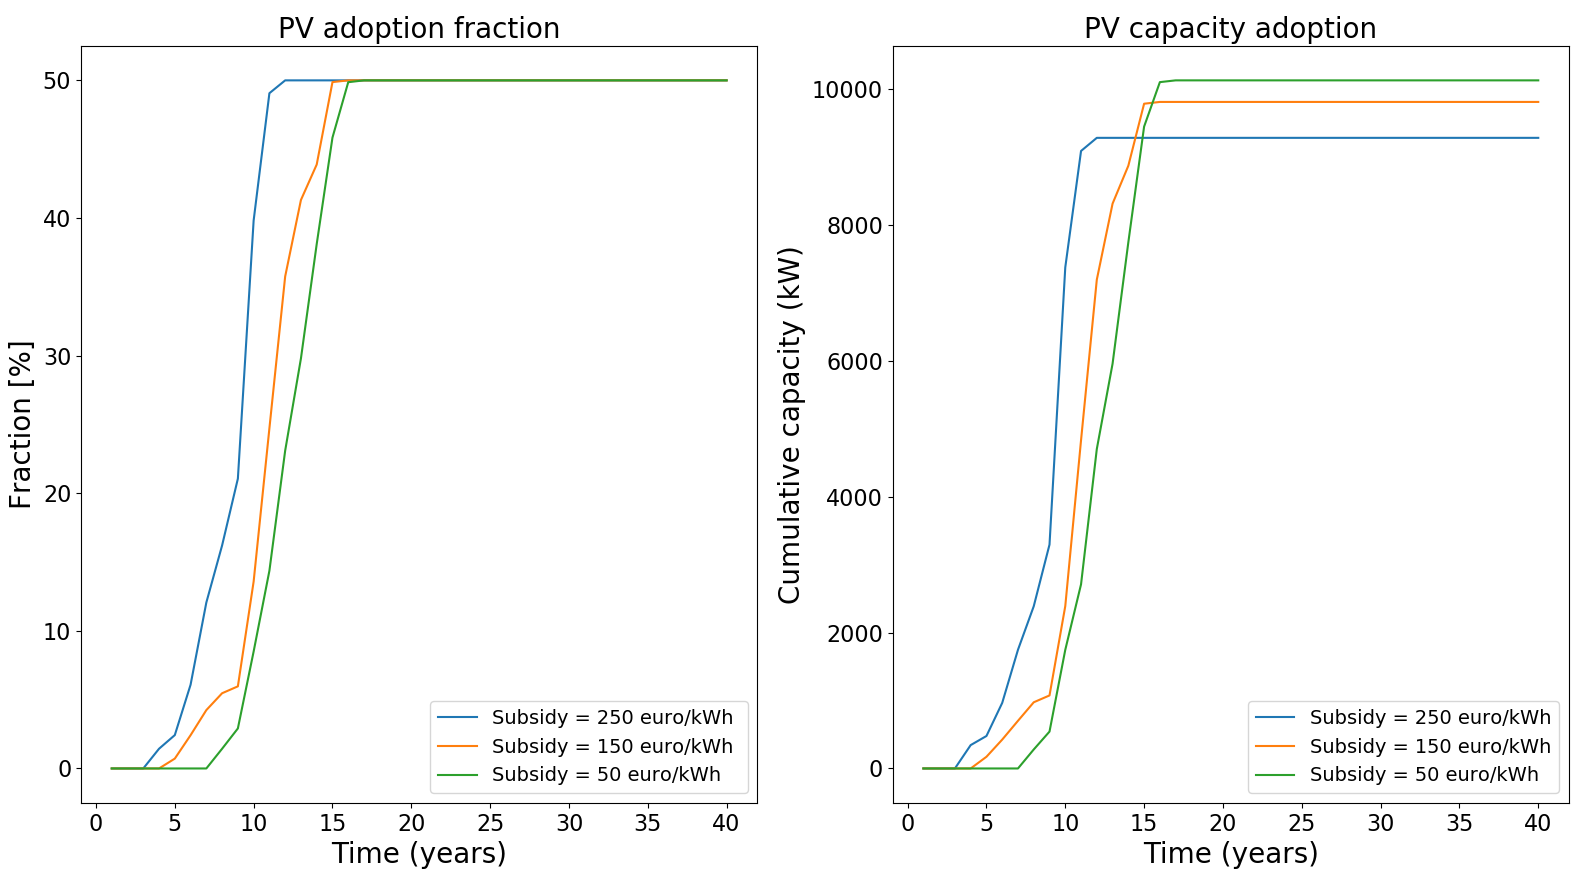
\includegraphics[width=10cm]{AppendixA/PVCapsubs.png}
    \caption{PV adoption for different battery subsides}
    \label{fig:}
\end{figure}
\noindent
\newline 
\begin{figure}[h!]
    \centering
    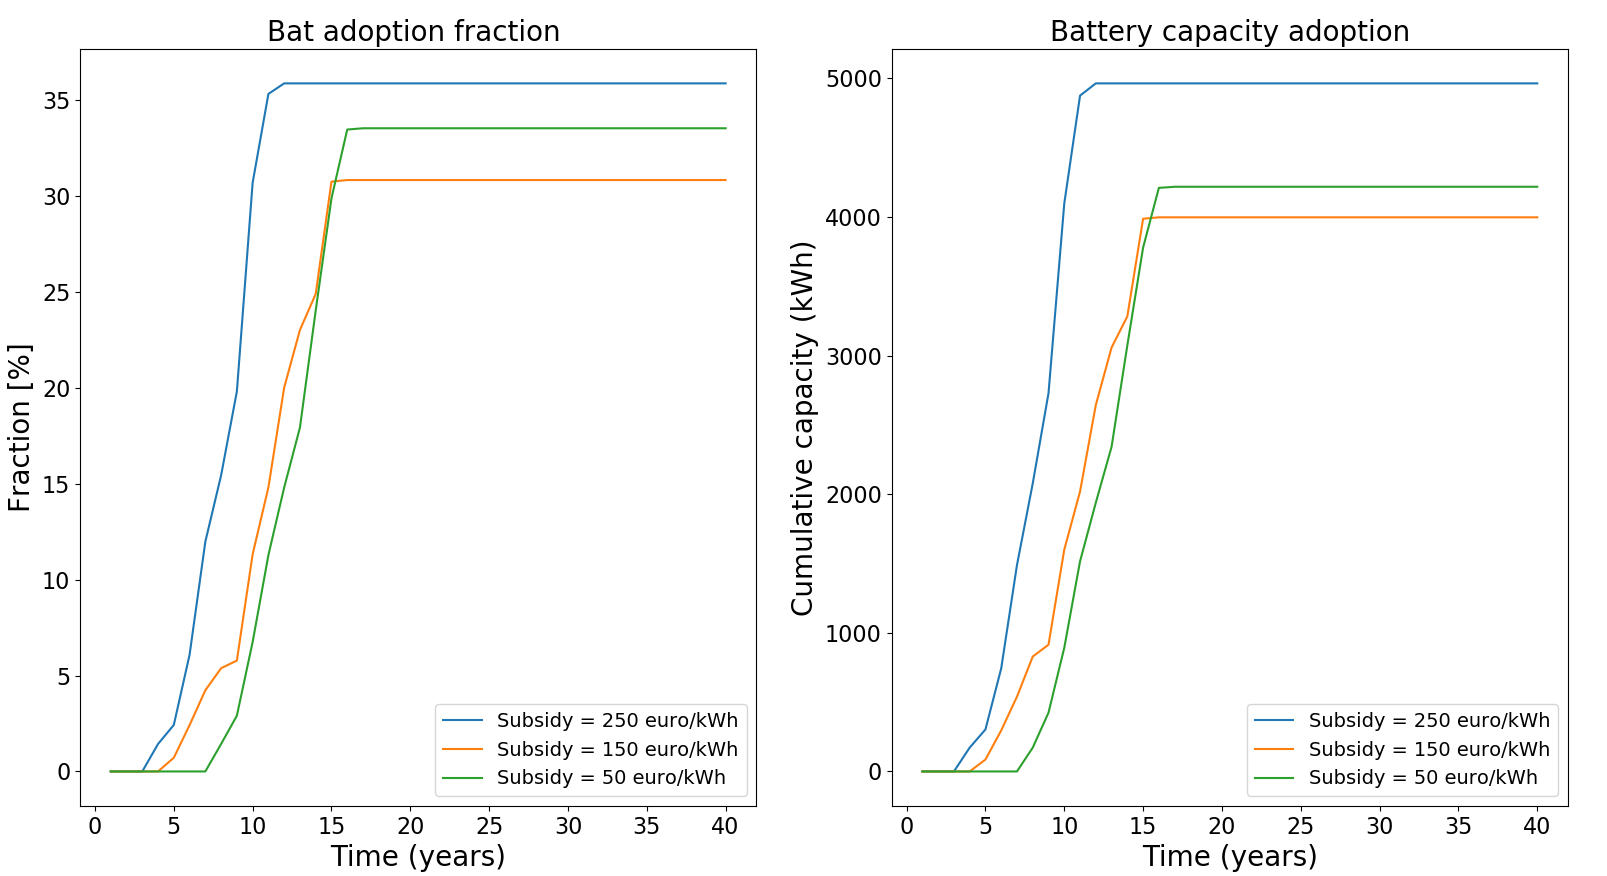
\includegraphics[width=10cm]{AppendixA/BatCapsubs.png}
    \caption{Battery adoption for different battery subsidies}
    \label{fig:}
\end{figure}
\noindent
\newline 
\begin{figure}[h!]
    \centering
    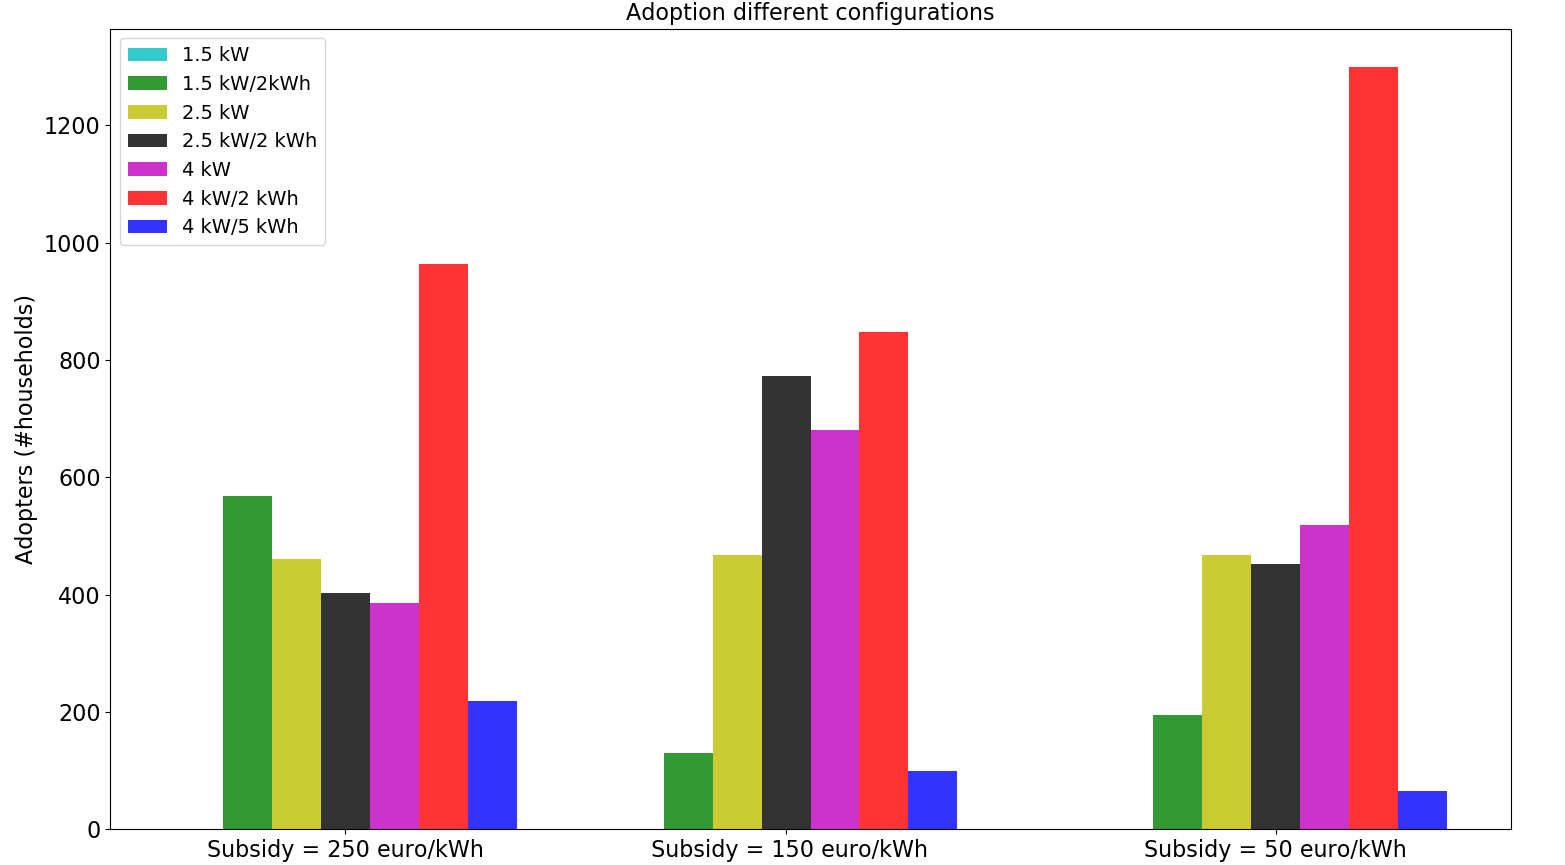
\includegraphics[width=10cm]{AppendixA/ConfigCapsubs.png}
    \caption{Configurations for different battery subsidies}
    \label{fig:}
\end{figure}
\noindent
\newline
\begin{figure}[h!]
    \centering
    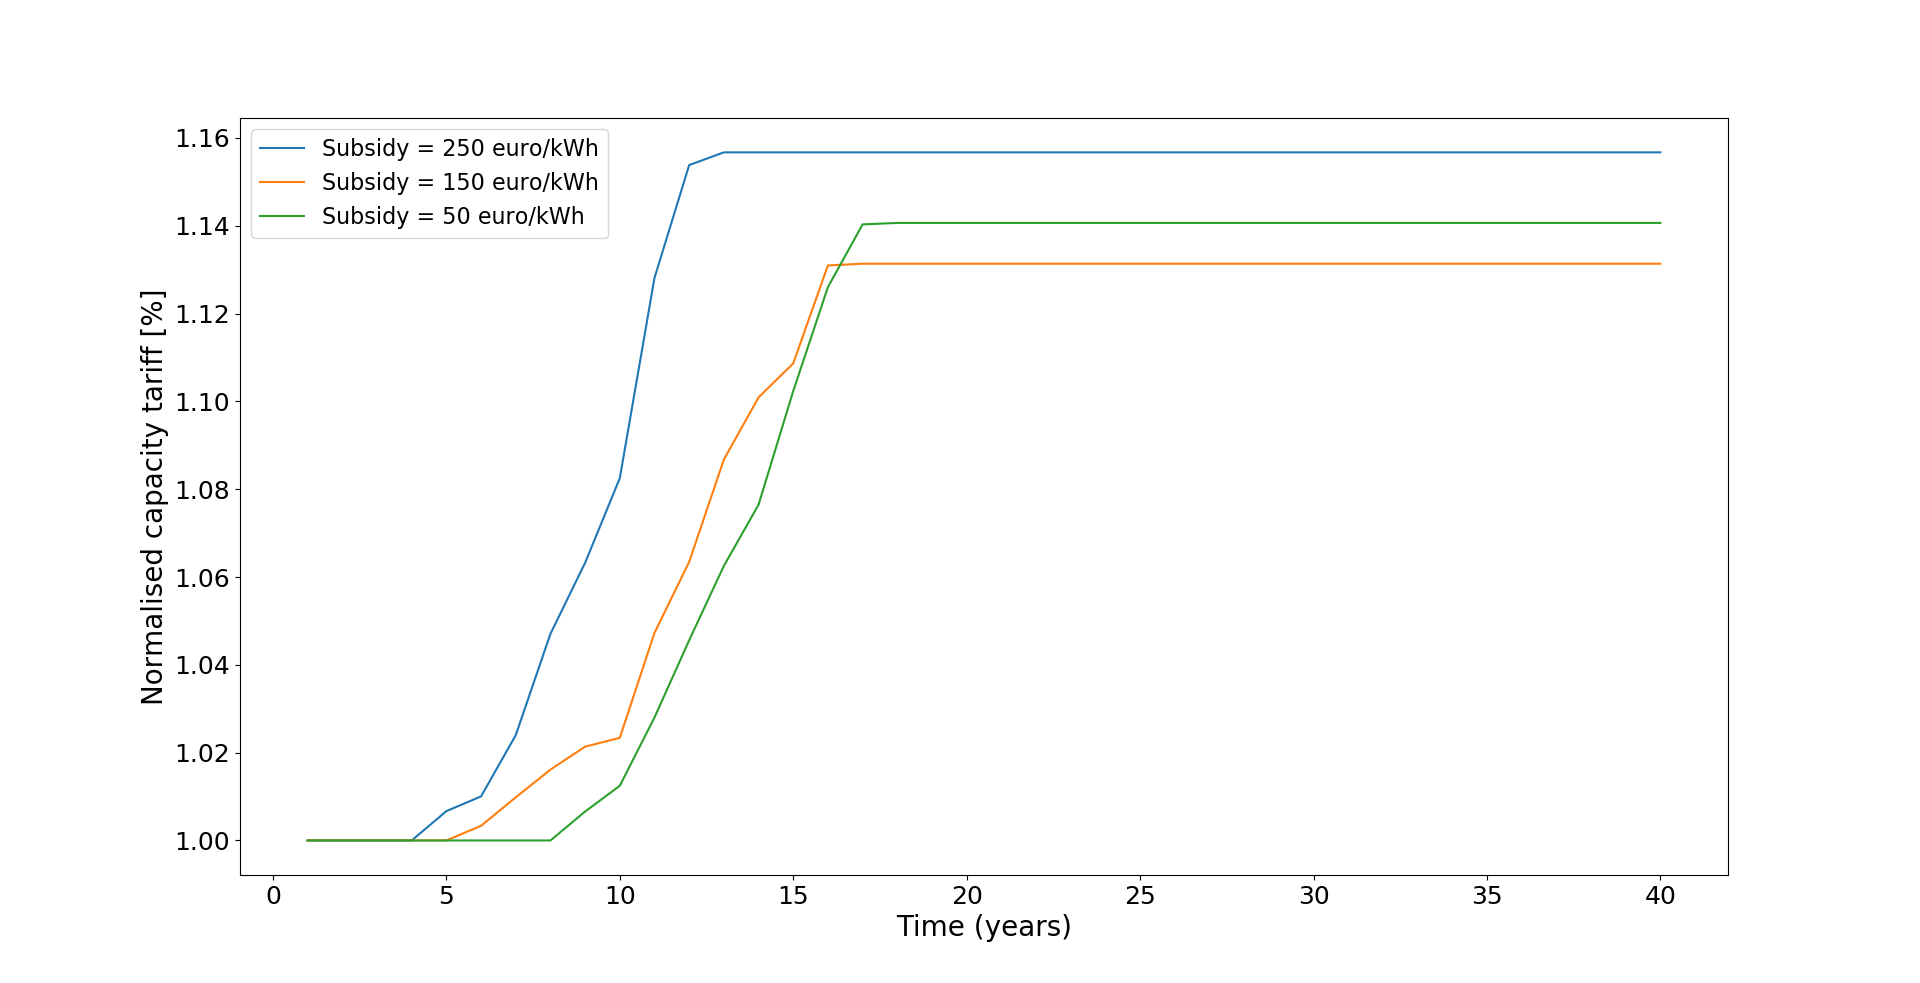
\includegraphics[width=10cm]{AppendixA/CapTarsubs.png}
    \caption{Normalised capacity tariff for different battery subsidies}
    \label{fig:}
\end{figure}
\newline
\subsection{Net billing}
The data for the 
\newline 
\begin{figure}[h!]
    \centering
    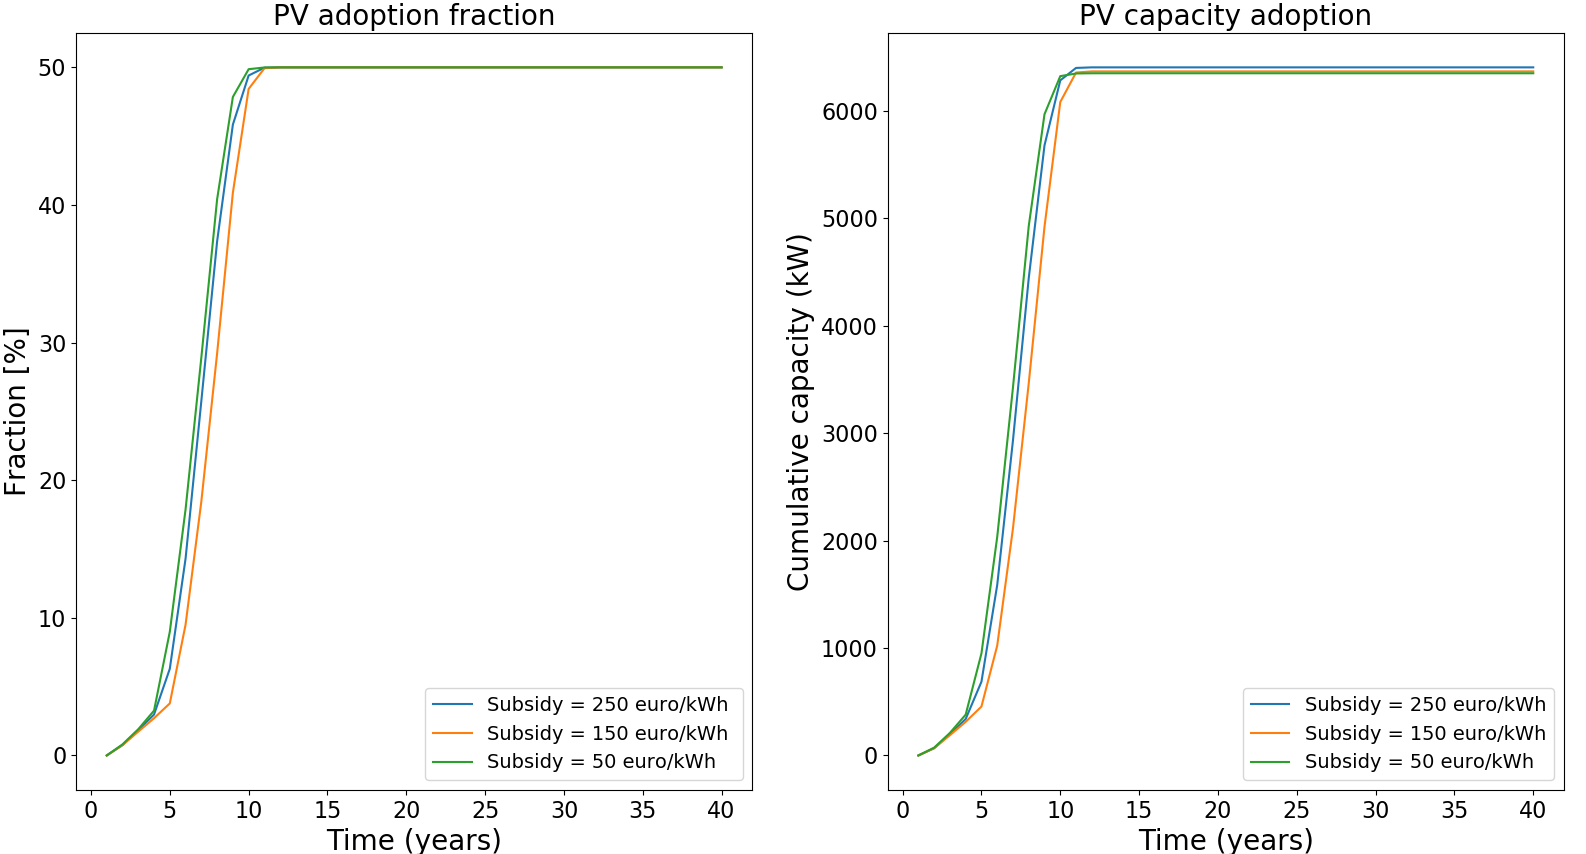
\includegraphics[width=10cm]{AppendixA/PVNBsubs.png}
    \caption{PV adoption for different subsidies}
    \label{fig:}
\end{figure}
\noindent
\newline 
\begin{figure}[h!]
    \centering
    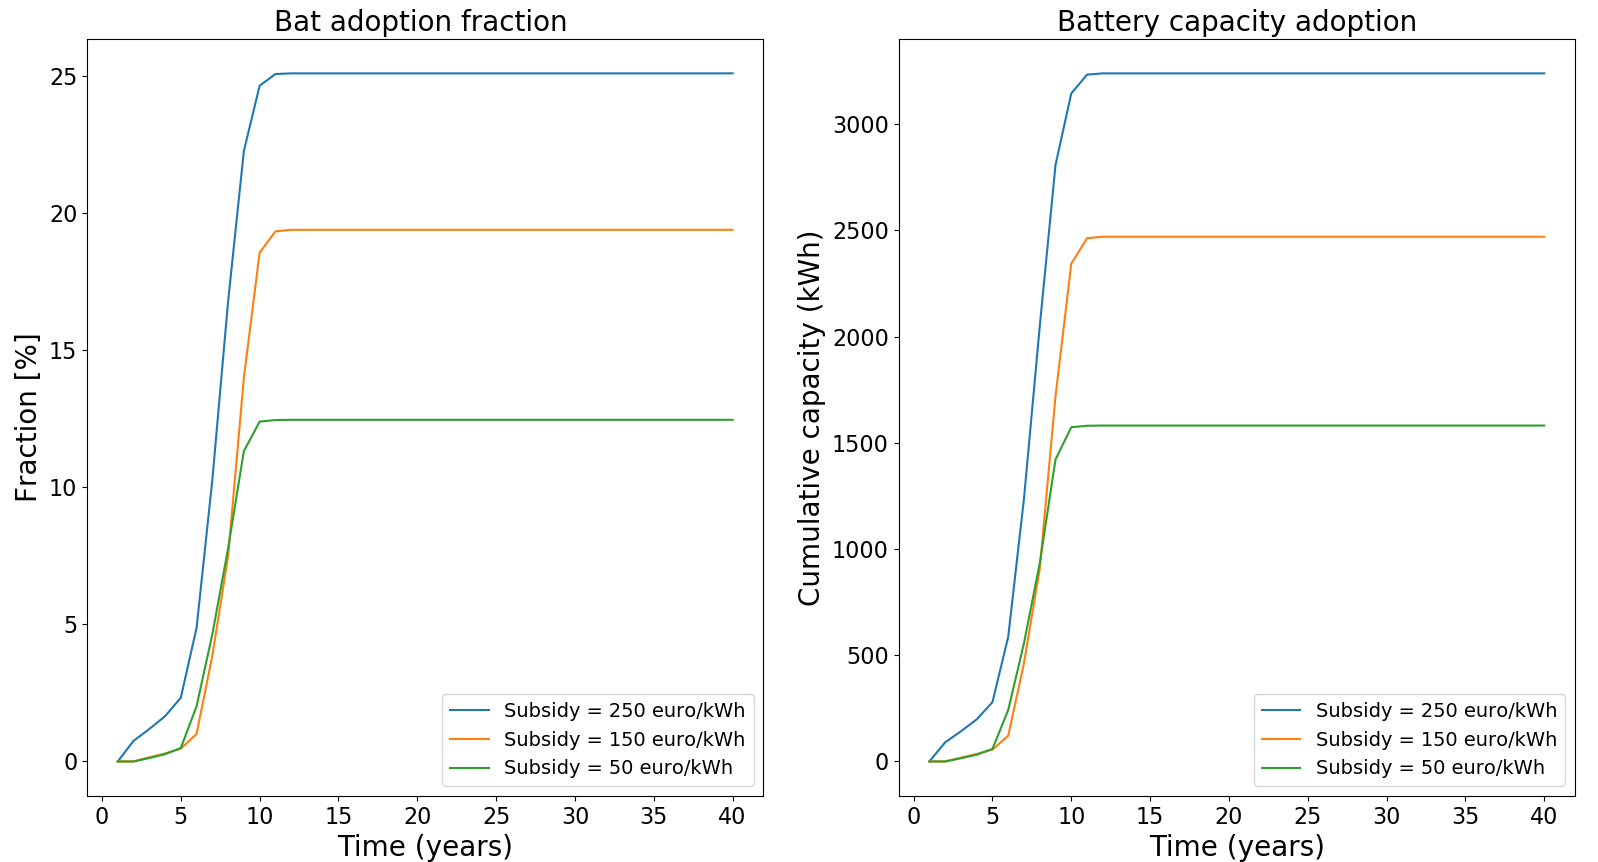
\includegraphics[width=10cm]{AppendixA/BatNBsubs.png}
    \caption{Battery adoption for different subsidies}
    \label{fig:}
\end{figure}
\noindent
\newline 
\begin{figure}[h!]
    \centering
    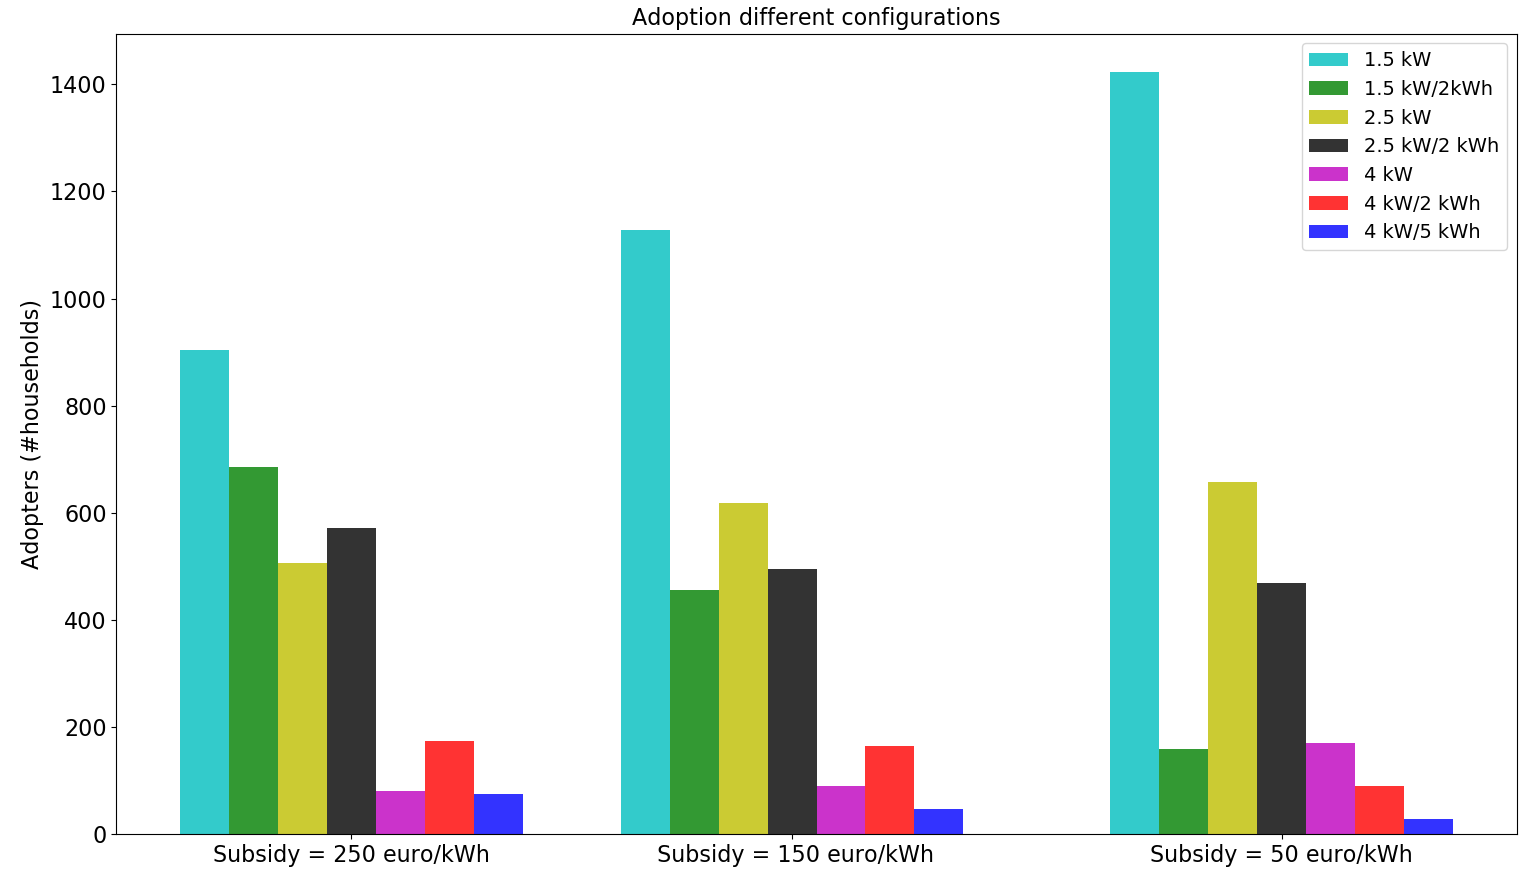
\includegraphics[width=10cm]{AppendixA/ConfigNBsubs.PNG}
    \caption{Configurations for different subsidies}
    \label{fig:}
\end{figure}
\noindent
\newline
\begin{figure}[h!]
    \centering
    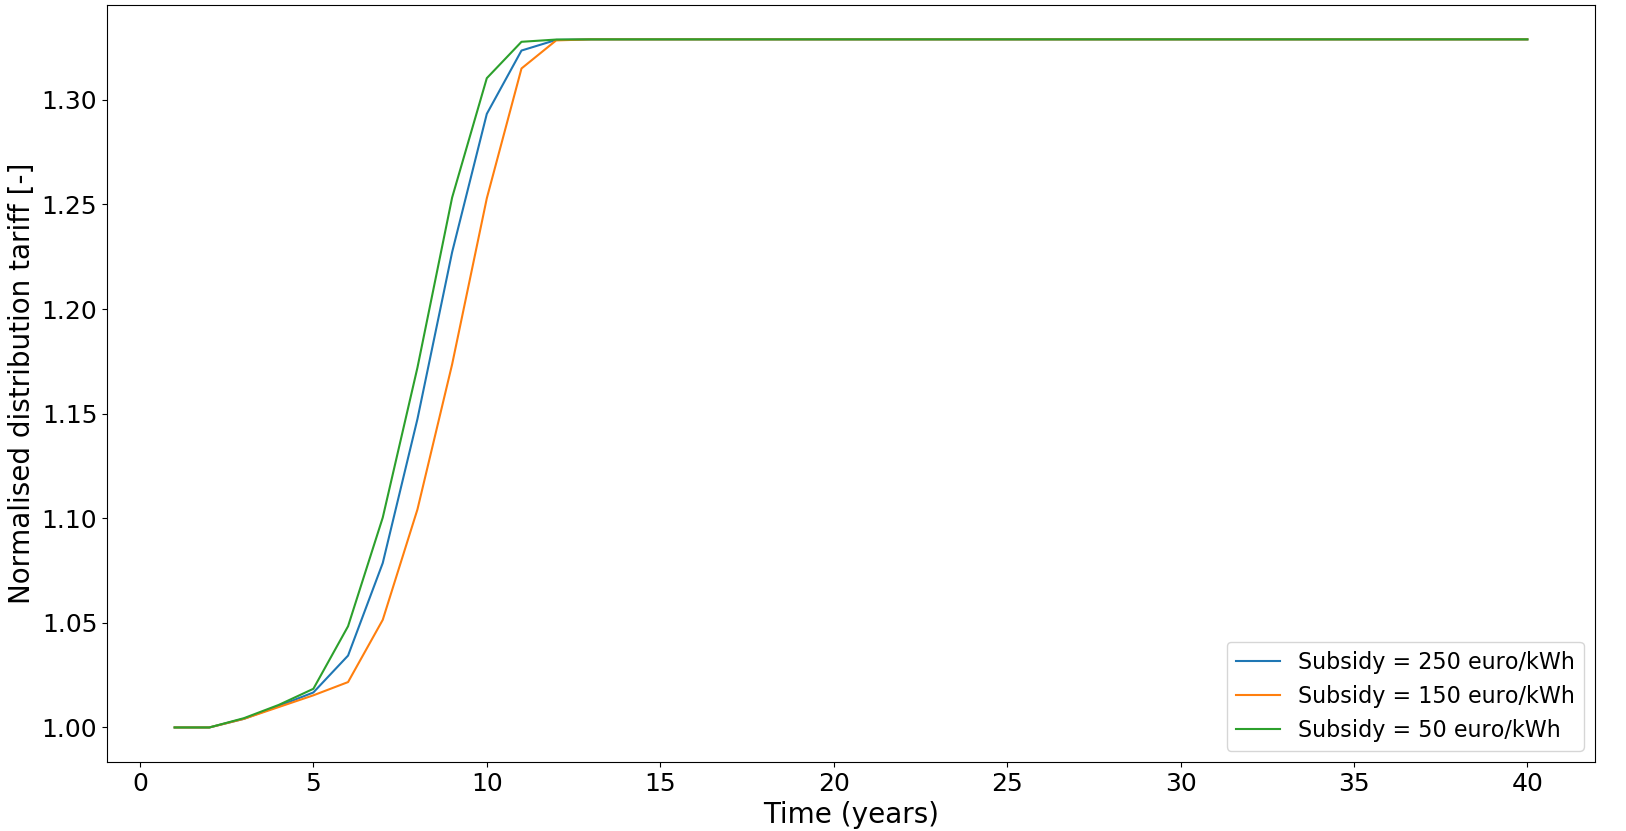
\includegraphics[width=10cm]{AppendixA/DistNBsubs.PNG}
    \caption{Normalised capacity tariff for different subsidies}
    \label{fig:}
\end{figure}
% ... en zo verder tot


\backmatter
% Na de bijlagen plaatst men nog de bibliografie.
% Je kan de  standaard "abbrv" bibliografiestijl vervangen door een andere.
\end{document}

%%% Local Variables: 
%%% mode: latex
%%% TeX-master: t
%%% End: 
